\documentclass[a4paper,12pt]{article}

\usepackage{fontspec}
\setmainfont{Times New Roman}
\usepackage{unicode-math}
\setmathfont{STIX Two Math}
\usepackage[margin=2.5cm,columnsep=0.8cm]{geometry}
\usepackage{microtype}
\usepackage{setspace}
\usepackage{lineno}
\usepackage{fancyhdr}
\usepackage{ragged2e}
\usepackage{graphicx}
\usepackage{placeins}
\usepackage{caption}
\DeclareCaptionFont{captionten}{\fontsize{10pt}{12pt}\selectfont}
\captionsetup{font={it,captionten},labelfont={bf,it},justification=centering,singlelinecheck=false}
\usepackage{booktabs}
\usepackage{tabularx}
\usepackage{array}
\usepackage{multirow}
\usepackage{xurl}
\usepackage[authoryear,round]{natbib}

\graphicspath{{../}}
\urlstyle{same}
\def\UrlFont{\rmfamily}
\renewcommand{\figurename}{Fig.}
\renewcommand{\topfraction}{0.95}
\renewcommand{\bottomfraction}{0.85}
\renewcommand{\textfraction}{0.05}
\renewcommand{\floatpagefraction}{0.85}
\makeatletter
\setlength{\@fptop}{0pt}
\setlength{\@fpsep}{10pt plus 2pt minus 2pt}
\setlength{\@fpbot}{0pt plus 1fil}
\makeatother

\setstretch{1.5}
\setlength{\parindent}{1.5em}
\setlength{\parskip}{0pt}

\pagestyle{fancy}
\fancyhf{}
\fancyfoot[C]{\thepage}
\renewcommand{\headrulewidth}{0pt}
\renewcommand{\footrulewidth}{0pt}

\renewenvironment{abstract}
  {\section*{Abstract}\noindent\ignorespaces}
  {\par\medskip}

\begin{document}

\title{\fontsize{16pt}{19.2pt}\selectfont\textbf{Beyond thermal accumulation: improving cross-regional grapevine phenology prediction with terrain-aware forcing and residual learning}}

\author{}
\date{}

\maketitle
\vspace{-2.0\baselineskip}

\begingroup
\setlength{\parindent}{0pt}
\setlength{\parskip}{0.35\baselineskip}
Linjia Yao\textsuperscript{a}, Qiang Yu\textsuperscript{b}, Gang Zhao\textsuperscript{b,*}

\textsuperscript{a} College of Natural Resources and Environment, Northwest A\&F University, Yangling 712100, China

\textsuperscript{b} State Key Laboratory of Soil and Water Conservation and Desertification Control, College of Soil and Water Conservation Science and Engineering, Northwest A\&F University, Yangling, Shaanxi 712100, China

\textsuperscript{*} Corresponding author: Gang Zhao, E-mail: gang.zhao@nwafu.edu.cn
\par
\endgroup

\linenumbers
\justifying

\begin{abstract}
Classical temperature-driven process models reduce phenological development to thermal accumulation toward fixed stage thresholds, assuming that temperature exposure and thermal responses remain sufficiently stable across sites and developmental stages. This simplification can generate spatially structured errors where terrain distorts gridded temperature estimates and later phenological stages respond to additional biophysical and management controls. To address these limitations, process-based phenology models were combined with terrain-adjusted temperature forcing and machine-learning residual correction. The framework was evaluated under nested spatially blocked validation using 23,170 TEMPO and DWD phenological records from 707 sites and 12,209 site-years during 1951--2026; machine-learning models were trained exclusively on spatially out-of-fold process-model residuals. The selected process models produced RMSE values of 9.6, 8.2, 15.5 and 30.5~d for budburst (BBCH07), flowering (BBCH65), veraison (BBCH81) and maturity/harvest (BBCH89), respectively. Terrain adjustment of ERA5-Land temperature produced limited changes for budburst and flowering but reduced RMSE by 1.3 and 2.2~d for veraison and maturity/harvest. Residual correction further reduced RMSE to 8.3, 7.7, 14.6 and 10.6~d, corresponding to improvements of 12.7\%, 6.0\%, 5.8\% and 65.4\%, respectively. MAE and RMSE decreased in all five held-out spatial test sets, and the pronounced late-season bias of the process-only maturity/harvest model was nearly eliminated. Ablation and SHAP analyses associated the corrections with process-model timing, temperature structure, terrain and spatial variability, atmospheric water demand and radiation. Thermal-time models therefore provide an interpretable biophysical foundation, while terrain-aware forcing and residual learning address complementary errors in environmental inputs and process representation. Their integration improves the accuracy and spatial transferability of grapevine phenology prediction, with the greatest benefit where systematic late-season errors remain.
\end{abstract}

\noindent\textit{Keywords:} Grapevine, Phenology, Terrain temperature correction, Process-based models, Machine learning, Cross-regional validation
\par\medskip

\section{Introduction}
\begingroup
\setlength{\parindent}{0pt}
\setlength{\parskip}{0.6\baselineskip}

Grapevine production is a globally important, high-value horticultural sector \citep{vanleeuwenClimateChangeImpacts2024}. Phenological stages mark key developmental windows and are therefore central to vineyard management and cross-regional coordination. Budburst, flowering, veraison, and maturity or harvest represent four major phenological stages. Shifts in their timing can alter the overlap between sensitive developmental periods and frost, heat, water deficit, pest and disease pressure, and vineyard operations, thereby affecting grape yield and fruit composition \citep{jonesClimateInfluencesGrapevine2000,tomasiGrapevinePhenologyClimate2011,garciadecortazar-atauriGrapevinePhenologyFrance2017}. Reliable and transferable phenology prediction is therefore important for seasonal climate-risk assessment, cross-regional vineyard management, planning for production-area shifts, and cultivar suitability evaluation.

Process-based phenology models translate environmental cues into development rates and predict an event when an accumulated state reaches a threshold \citep{chuineProcessBasedModelsPhenology2017}. Most operational grapevine models implement this idea as a temperature-driven clock. Growing degree-day (GDD) models and the Grapevine Flowering Veraison (GFV) model accumulate heat from a fixed date until a stage-specific thermal requirement is reached \citep{garciadecortazar-atauriPerformanceSeveralModels2009,parkerGeneralPhenologicalModel2011a}. Budburst models additionally represent winter dormancy by coupling chilling and forcing sequentially, in parallel or with partial overlap. In biological terms, chilling promotes the transition from endodormancy, when buds cannot resume growth under favourable conditions, to ecodormancy, when growth becomes responsive to spring warmth; greater chilling generally reduces the subsequent heat requirement \citep{chuineUnifiedModelBudburst2000,fadonConceptualFrameworkWinter2020}. These models are parsimonious and interpretable, but chilling units, forcing rates and thermal thresholds are proxies for latent developmental states rather than direct physiological measurements. Dormancy also involves transport, phytohormones, genetic and epigenetic regulation, and carbohydrate dynamics \citep{fadonConceptualFrameworkWinter2020}. Consequently, alternative temperature functions can imply different physiology: seven of twelve evaluated chilling models produced an implausible chilling--heat relationship and biased warming projections \citep{wangOverestimationEffectClimatic2020}.

Grapevine phenology models commonly calibrate cultivar-specific thermal requirements, yet apply these requirements as fixed parameters across years and environments \citep{parkerAdaptationClimateChange2020,tanOvercomingMechanisticLimitations2024a,thomasDevelopingTestingWinegrape2026}. Such formulations relate development primarily to current weather and do not explicitly represent adaptive changes or the effects of preceding environmental conditions on subsequent developmental rates \citep{kangPerformanceNineMaize2024,wuNecessityCouplingLegacy2024}. Models that begin thermal accumulation on fixed calendar dates additionally assume that vines enter the accumulation period at comparable physiological states \citep{filaComparisonDifferentModelling2014,parkerAdaptationClimateChange2020}. Phase-to-phase formulations improve synchronization with observed plant development \citep{deresseguierModelingGrapevinePhenology2026,thomasDevelopingTestingWinegrape2026}. These assumptions incompletely represent how cultivar- and stage-specific developmental states respond to weather. Experimental evidence indicates that temperature effects can be nonlinear and interact with water supply, source--sink balance and cultivar \citep{sadrasNonlinearEffectsElevated2013,cameronEffectTemperatureGrapevine2022}. Maturity/harvest is especially difficult because the recorded event may reflect sugar or acidity targets and management decisions, whereas berry ripening and composition respond jointly to temperature, water and nitrogen status, radiation, crop load and cultural practices \citep{parkerAdaptationClimateChange2020,vanleeuwenClimateChangeImpacts2024}. Thus, one thermal requirement cannot be assumed to encode the same physiological meaning for budburst, flowering, veraison and maturity/harvest across regions.

Recent evidence confirms that this limitation is not resolved by parameter calibration alone. Environmental clustering reduced heterogeneity in thermal requirements and improved twelve crop phenology models, indicating that unrepresented adaptation can be absorbed into apparently constant parameters \citep{tanOvercomingMechanisticLimitations2024a}. Non-constant formulations reduced systematic bias under historical climate change \citep{kangPerformanceNineMaize2024}, while coupling legacy effects with temperature response showed that development depends partly on preceding environmental conditions rather than current temperature alone \citep{wuNecessityCouplingLegacy2024}. For grapevine, published models calibrated mainly in Europe performed poorly across Australian regions until thermal requirements and response functions were re-estimated; using the preceding observed phenophase further improved prediction, and harvest remained the least accurate stage \citep{thomasDevelopingTestingWinegrape2026}. More flexible dormancy models provide a related advance: PhenoFlex connects Dynamic Model chilling with growing-degree-hour forcing through a flexible transition, although physiologically unrealistic fitted responses, warm-winter performance and sensitivity to calibration-data diversity still constrain transfer \citep{luedelingPhenoFlexIntegratedModel2021,fernandezUnusuallyWarmWinter2022,picornellInfluenceCalibrationData2025,mojahidCrossRegionalValidation2025}.

The second central limitation is the weather forcing supplied to the model. Viticulture is intrinsically local and scale dependent: elevation, slope, aspect, cold-air drainage, radiation exposure, surrounding land cover and canopy structure can generate contrasting temperatures over short distances \citep{neethlingSpatialComplexityTemporal2019}. In a 19,233-ha Bordeaux vineyard area, 90 in-canopy sensors recorded daily minimum-temperature differences of up to 10~\(^{\circ}\)C and within-vintage differences of about 320 degree-days in the Winkler index; these temperature patterns were related to terrain and produced spatial differences in grapevine phenology \citep{deresseguierTemperatureVariabilityLocal2020}. Recent local-scale modelling likewise found that phenophase-based models transferred better than fixed-date alternatives and that model projections diverged more strongly under larger warming increments \citep{deresseguierModelingGrapevinePhenology2026}. Gridded meteorological products can therefore be internally consistent yet fail to represent the thermal environment experienced at a vineyard site. Elevation-based temperature adjustment addresses one major component of this scale mismatch, but its benefit must be quantified because aspect, cold-air pooling and canopy energy balance are not reducible to elevation alone.

These two limitations generate different but interacting errors. Process-based phenology models retain an interpretable developmental baseline; terrain adjustment targets error in meteorological forcing; and residual learning can represent repeatable discrepancies associated with omitted environmental and spatial controls without claiming that the data-driven component identifies the missing physiology. Physics-guided continuous learning and other process--data hybrids support this division of roles \citep{reichsteinDeepLearningProcess2019,ouContinuousLearningFramework2025}. Random validation can overestimate predictive performance when nearby observations share similar climate and terrain conditions, because environmentally similar records may occur in both training and test sets. Both process-model selection and residual correction therefore require testing in held-out regions \citep{robertsCrossvalidationStrategiesData2017,valaviBlockCVPackageGenerating2019}.

This study therefore evaluates whether process-based phenology modelling across four developmental stages, terrain-adjusted temperature forcing and machine-learning residual correction improve the accuracy and spatial transferability of grapevine phenology prediction. Raw and adjusted temperature branches are compared within nested spatial validation, residual learners are trained only on out-of-fold process-model errors, and the resulting gains are examined through temperature-input sensitivity and mechanism-group ablation.

\endgroup
\section{Materials and methods}

\begingroup
\setlength{\parindent}{0pt}
\setlength{\parskip}{0.5\baselineskip}

\subsection{Study framework}

The overall study framework is shown in Fig.~\ref{fig:study_framework}. The analysis separated the contributions of the process-model baseline, elevation adjustment of thermal forcing and residual correction using antecedent weather and terrain covariates. Phenological observations, raw ERA5-Land meteorological forcing, digital elevation model (DEM) terrain information and the corresponding elevation-adjusted temperature series were first organized as model inputs. Candidate process models were evaluated for each of the four main BBCH phenological stages. Within each outer spatial split, calibration, residual learning and model selection were restricted to the spatial training blocks, and inner spatial out-of-fold process-model residuals defined the residual-learning task. The held-out outer spatial blocks were used only for final evaluation.

\begin{figure}[!p]
\centering
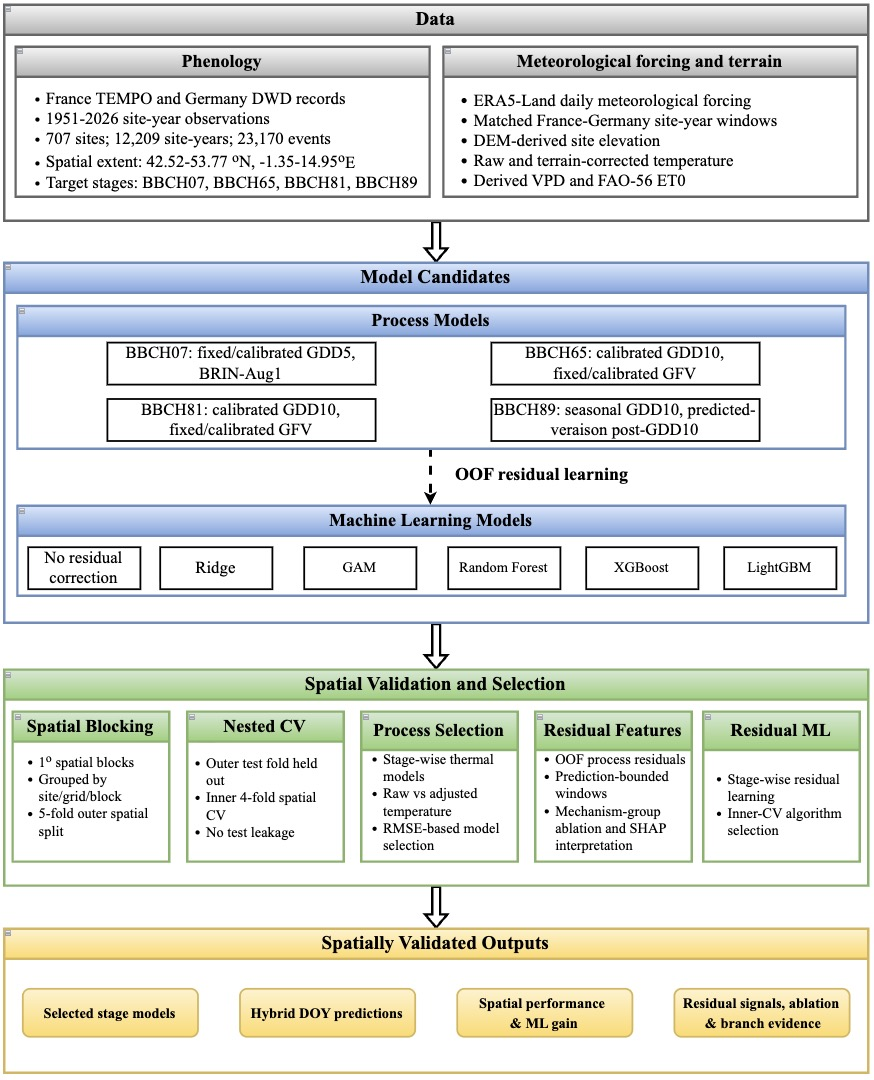
\includegraphics[width=\textwidth,height=0.86\textheight,keepaspectratio]{fig/workflow/grape_phenology_workflow.png}
\caption{Workflow of this study. OOF, out-of-fold. CV, cross-validation. VPD, vapour pressure deficit. ET0, FAO-56 reference evapotranspiration.}
\label{fig:study_framework}
\end{figure}

\FloatBarrier

\subsection{Study area and datasets}

\subsubsection{Source datasets and study area}

The study used two public grapevine phenology datasets from France and Germany. French records were downloaded from the TEMPO phenological database public API (\url{https://data.pheno.fr/api/}). German records were downloaded from the Deutscher Wetterdienst (DWD, German Weather Service) open-data phenology archive (\url{https://opendata.dwd.de/climate_environment/CDC/observations_germany/phenology/}). Both source datasets include event dates, observation years, site identifiers and geographic coordinates. TEMPO records provide explicit BBCH codes, which were directly normalized to two-digit BBCH stages. DWD records use DWD stage names and identifiers, but the selected grapevine phases have the same phenological meaning as the target BBCH stages. These stages were therefore mapped to the corresponding extended BBCH stages following the grapevine BBCH standard \citep{lorenzGrowthStagesGrapevine1995}. This harmonization provided a common stage framework for cross-source analysis. The site inventory used for data screening and blocked spatial validation contained 1,624 French sites and 700 German sites distributed across lowland, valley and upland terrain (Fig.~\ref{fig:study_area_sites}). Site elevation and local terrain information were derived from the Copernicus GLO-30 digital elevation model (DEM; \url{https://registry.opendata.aws/copernicus-dem/}).

\begin{figure}[!htb]
\centering
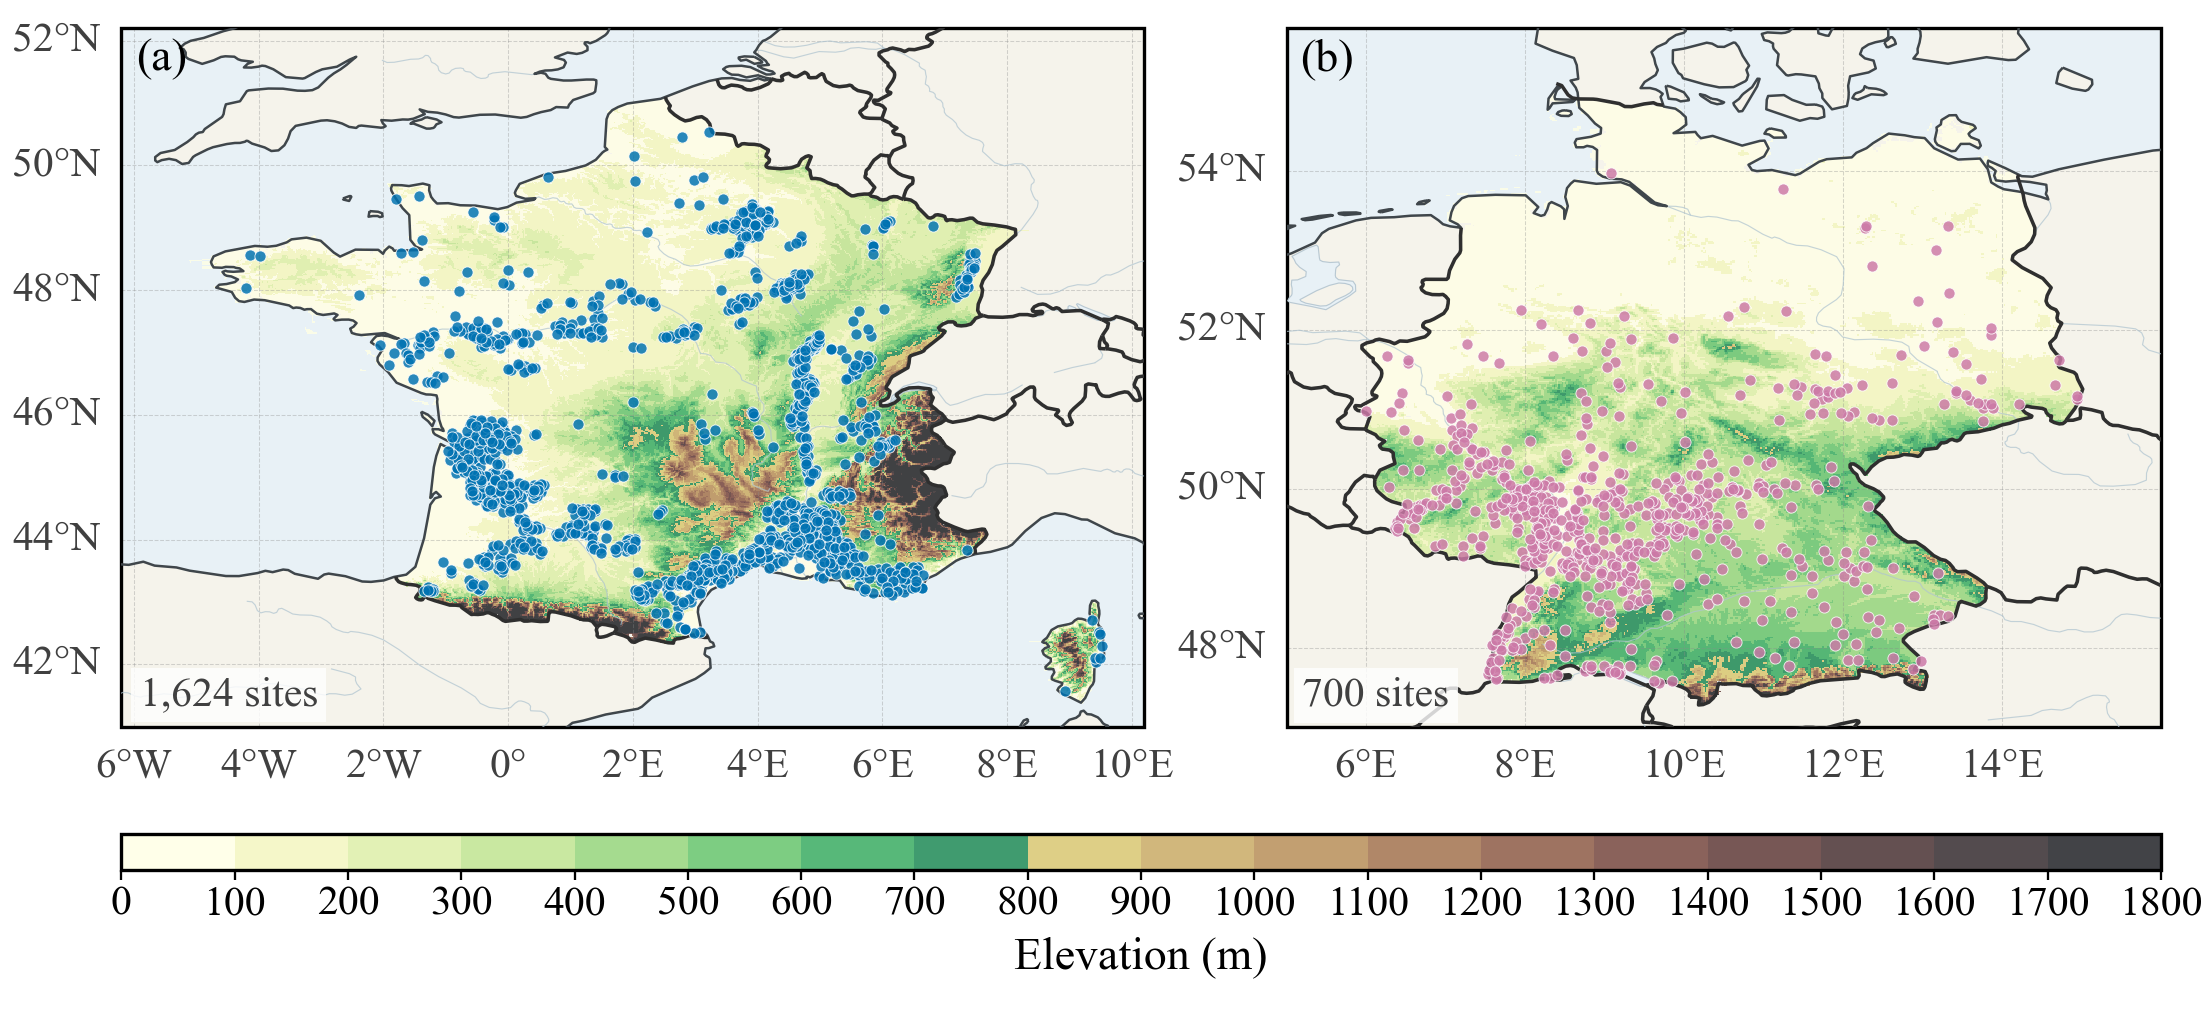
\includegraphics[width=\textwidth]{fig/phenology_distribution/france_germany_four_stage_site_distribution_dem_overlap.png}
\caption{Spatial distribution of grapevine phenology observation sites in France and Germany.}
\label{fig:study_area_sites}
\end{figure}

\FloatBarrier

\subsubsection{Event aggregation and main analysis sample}

The event-level analysis unit was a site--year--stage record. The target stages were BBCH07 (budburst), BBCH65 (flowering), BBCH81 (veraison), and BBCH89 (maturity/harvest). Duplicate source records were removed before harmonization. When multiple observations remained for the same source, site, year and target stage, BBCH07 and BBCH81 were represented by the earliest recorded date because both denote the onset of a transition, whereas BBCH65 and BBCH89 were represented by the median date. The number and range of contributing observations were retained as quality-control fields.

BBCH81 records underwent an additional harmonization audit because the French and German sources use related but not identical operational definitions of veraison onset. Exact BBCH81 observations were retained; German records with DWD date-quality flags 5 (doubtful) or 8 (incorrect) were excluded. The earliest eligible BBCH81 date was used for each site--year, and events were excluded when the range among eligible dates exceeded 21~d or when the date did not follow flowering or precede maturity/harvest where those adjacent stages were observed. This audit retained 6,364 of 6,394 BBCH81 events and did not alter the predefined spatial-fold assignments.

Each retained event was represented by its observed day of year (DOY), site identifier, year, geographic coordinates, source dataset and target BBCH stage. Records with high-confidence BBCH mapping and at least 10 years of observations for the corresponding site--stage were classified as core; records with high- or medium-confidence mapping and at least 5 years were classified as extended; all remaining records formed a sensitivity tier. The process-model analysis pooled the core and extended tiers, excluded sensitivity-tier records and non-increasing observed stage sequences, and required complete physically plausible weather through the observed event, stable site coordinates, DEM-derived site elevation, ERA5-Land grid elevation and unique point-weather matching. These criteria produced a process-model foundation dataset of 23,671 events from 707 sites and 12,625 site-years. The residual-learning sample further required a valid process-model prediction and complete retained predictors, resulting in 23,170 events from 707 sites and 12,209 site-years during 1951--2026, spanning 42.52--53.77$^\circ$N and -1.35--14.95$^\circ$E. Event counts by stage are reported in Table~\ref{tab:main_analysis_stage_counts}.

\begin{table}[!htb]
\centering
\caption{Stage-specific event counts in the final main-analysis sample after residual-learning eligibility filtering.}
\label{tab:main_analysis_stage_counts}
\fontsize{10pt}{12pt}\selectfont
\setlength{\tabcolsep}{4pt}
\begin{tabularx}{\textwidth}{>{\raggedright\arraybackslash}p{0.20\textwidth}
>{\raggedright\arraybackslash}X
>{\raggedleft\arraybackslash}p{0.18\textwidth}}
\toprule
Target stage & Phenological event & Events (n) \\
\midrule
BBCH07 & Budburst & 3,646 \\
BBCH65 & Flowering & 4,288 \\
BBCH81 & Veraison & 4,325 \\
BBCH89 & Maturity/harvest & 10,911 \\
Total & & 23,170 \\
\bottomrule
\end{tabularx}
\end{table}


\subsection{Meteorological forcing and terrain-based temperature correction}

Daily meteorological forcing was obtained through Google Earth Engine from the ERA5-Land Daily Aggregated collection (collection ID: \url{ECMWF/ERA5_LAND/DAILY_AGGR}) on its 0.1$^\circ$ grid \citep{munozSabaterERA5Land2021,copernicusClimateChangeServiceERA5LandHourly2019}. Each site was matched to the nearest ERA5-Land grid centre. Site--year series extended from 1 August of the preceding year to 31 December of the target year and included daily mean, minimum and maximum 2-m air temperature, 2-m dew-point temperature, total precipitation, surface pressure, downward surface shortwave radiation and 10-m wind components. Quality control required unique dates, complete variables through the observed event, minimum temperature no greater than mean temperature, mean temperature no greater than maximum temperature, and no materially negative precipitation or radiation.

Site terrain was derived from the approximately 30-m Copernicus GLO-30 DEM. Site elevation was sampled at the central pixel, slope and aspect were calculated from the local 3~$\times$~3-pixel gradient, and local elevation variability was represented by the standard deviation within an 11~$\times$~11-pixel window. Northness was calculated as the cosine of aspect. ERA5-Land grid elevation was calculated from the invariant geopotential field using standard gravity. Because vineyard sites are distributed across heterogeneous terrain, DEM-derived site elevation was used to adjust ERA5-Land daily air-temperature series from the matched grid-cell elevation to the site elevation. Elevation-based temperature adjustment is a common method for adapting gridded climate fields to terrain-dependent local temperature conditions \citep{dalyPhysiographicallySensitiveMapping2008}. The standard-atmosphere lapse rate of 6.5~\(^{\circ}\)C km\(^{-1}\) was used as the correction parameter \citep{isoStandardAtmosphere1975}:

\begin{equation}
T_{adj,d}=T_{raw,d}-\gamma\left(z_{site}-z_{grid}\right), \quad \gamma=0.0065~^{\circ}\mathrm{C}~\mathrm{m}^{-1}
\label{eq:temperature_adjustment}
\end{equation}

where \(T_{adj,d}\) and \(T_{raw,d}\) are the elevation-adjusted and raw temperatures on day \(d\), respectively; \(z_{site}\) and \(z_{grid}\) are the DEM-derived site elevation and matched ERA5-Land grid-cell elevation; and \(\gamma\) is the fixed lapse rate.

The correction was applied consistently to daily mean, minimum and maximum temperature. Non-temperature meteorological variables were taken directly from the matched ERA5-Land grid cell. Elevation was the only terrain variable used to modify temperature directly; northness and local elevation variability were available only to the residual-learning component. Raw-temperature and elevation-adjusted-temperature branches used identical observations and spatial folds; where calibration was required, process-model parameters were estimated independently within each branch. Their comparison therefore quantified the predictive value of elevation adjustment after branch-specific calibration rather than a same-parameter physical counterfactual.

\subsection{Candidate process-based phenology models}

All four target stages were modelled within a general temperature-driven accumulation-and-threshold framework. Candidate formulations represented the different physiological controls on dormancy release, reproductive development, berry ripening and maturity/harvest. Parameters were specified or calibrated by stage. Every calibrated parameter set was shared by all sites and years of that stage within the active training partition and was held fixed when predicting the corresponding validation or test partition. Cultivar-, site- and year-specific recalibration was not performed. For GDD-type cumulative forcing models, daily effective thermal forcing was calculated as:

\begin{equation}
GDD_d=\max\left(T_{\mathrm{mean},d}-T_b,0\right)
\label{eq:gdd}
\end{equation}

The predicted event date was the first day on which accumulated forcing reached a stage-specific threshold.

For BBCH07, fixed-parameter GDD5, calibrated GDD5 and the BRIN chilling--forcing model were compared. GDD5 served as a conventional thermal-time benchmark for grapevine budburst. BRIN represented an established two-step budburst framework \citep{garciadecortazar-atauriPerformanceSeveralModels2009}, consistent with the unified budburst modelling framework of \citet{chuineUnifiedModelBudburst2000}. BRIN used a Bidabe chilling coefficient of 2.17, a forcing base temperature of 5~\(^{\circ}\)C and an upper forcing-response temperature of 25~\(^{\circ}\)C; chilling and forcing thresholds were estimated within the active training partition.

For BBCH65 and BBCH81, GDD10 was used as a standard grapevine thermal-time comparator \citep{zapataPredictingKeyPhenological2017}. The Grapevine Flowering Veraison (GFV) model was also included for flowering and veraison of \textit{Vitis vinifera}, using the fixed DOY 60 start and 0~\(^{\circ}\)C base temperature proposed by \citet{parkerGeneralPhenologicalModel2011a}.

For BBCH89, GDD10 accumulation was started either on 1 January or from the fold-specific process-predicted BBCH81 date. This stage-to-stage accumulation setting follows previous cumulative degree-day applications to post-veraison berry development and harvest-related stages \citep{molitorHighResolutionCumulativeDegree2014,zapataPredictingKeyPhenological2017}. Literature-derived fixed thresholds served only as external transfer benchmarks; final process-model selection was restricted to formulations calibrated within the training partitions.

\begin{table}[!htb]
\centering
\caption{Candidate process models evaluated for the four target grapevine phenological stages.}
\label{tab:process_model_candidates}
\fontsize{9pt}{11pt}\selectfont
\renewcommand{\arraystretch}{1.12}
\setlength{\tabcolsep}{4pt}
\begin{tabularx}{\textwidth}{>{\centering\arraybackslash}p{0.12\textwidth}
>{\raggedright\arraybackslash}p{0.22\textwidth}
>{\raggedright\arraybackslash}p{0.36\textwidth}
>{\raggedright\arraybackslash}X}
\toprule
Stage & Candidate model & Start and thermal response & Calibrated parameters \\
\midrule
\multirow[c]{3}{=}{BBCH07} & Fixed GDD5 & 1 January, \(T_b=5~^{\circ}\)C & None \\
 & Calibrated GDD5 & 1 January, \(T_b=5~^{\circ}\)C & Forcing threshold \(F^*\) \\
 & BRIN-Aug1 & Previous 1 August, chilling and forcing phases & Chilling and forcing thresholds \\
\addlinespace[2pt]
\multirow[c]{3}{=}{BBCH65} & Calibrated GDD10 & 1 January, \(T_b=10~^{\circ}\)C & Forcing threshold \(F^*\) \\
 & Fixed GFV & DOY 60, \(T_b=0~^{\circ}\)C & None \\
 & Calibrated GFV & DOY 60, \(T_b=0~^{\circ}\)C & Forcing threshold \(F^*\) \\
\addlinespace[2pt]
\multirow[c]{3}{=}{BBCH81} & Calibrated GDD10 & 1 January, \(T_b=10~^{\circ}\)C & Forcing threshold \(F^*\) \\
 & Fixed GFV & DOY 60, \(T_b=0~^{\circ}\)C & None \\
 & Calibrated GFV & DOY 60, \(T_b=0~^{\circ}\)C & Forcing threshold \(F^*\) \\
\addlinespace[2pt]
\multirow[c]{2}{=}{BBCH89} & Seasonal GDD10 & 1 January, \(T_b=10~^{\circ}\)C & Forcing threshold \(F^*\) \\
 & Post-veraison GDD10 & Fold-specific predicted BBCH81 date, \(T_b=10~^{\circ}\)C & Forcing threshold \(F^*\) \\
\bottomrule
\end{tabularx}
\parbox{\textwidth}{\footnotesize GDD5 and GDD10, growing degree days above base temperatures of 5 and 10~\(^{\circ}\)C, respectively; GFV, Grapevine Flowering Veraison; DOY, day of year; \(T_b\), base temperature; \(F^*\), forcing threshold.}
\end{table}

\subsection{Candidate machine-learning residual models}

Machine learning was used as a residual-learning component rather than as a direct phenology-date model. For event \(i\), the signed residual and the resulting hybrid prediction were defined as:

\begin{equation}
\begin{alignedat}{2}
r_i \quad &={} \quad DOY_{\mathrm{obs},i}-\widehat{DOY}_{\mathrm{proc},i},\\
\widehat{DOY}_{\mathrm{hyb},i} \quad &={} \quad \widehat{DOY}_{\mathrm{proc},i}+\widehat{r}_i
\end{alignedat}
\label{eq:residual_hybrid}
\end{equation}

Positive residuals indicate observed events later than the process-model prediction, whereas negative residuals indicate earlier observed events.

The candidate machine-learning models were selected to span simple shrinkage, smooth additive response and tree-ensemble structures (Table~\ref{tab:residual_ml_candidates}). Ridge regression provided a regularized linear benchmark. The GAM implementation represented additive nonlinear responses using spline-expanded predictors with ridge penalization. Random forest, XGBoost and LightGBM represented increasingly flexible tree-ensemble models. All candidate machine-learning models were applied to the same signed-residual target and were combined with the selected process-model prediction in the same hybrid form.

\begin{table}[!htb]
\centering
\caption{Candidate machine-learning models used for residual learning in the hybrid framework.}
\label{tab:residual_ml_candidates}
\fontsize{9pt}{11pt}\selectfont
\renewcommand{\arraystretch}{1.12}
\setlength{\tabcolsep}{4pt}
\begin{tabularx}{\textwidth}{>{\raggedright\arraybackslash}p{0.16\textwidth}
>{\raggedright\arraybackslash}p{0.20\textwidth}
>{\raggedright\arraybackslash}p{0.37\textwidth}
>{\raggedright\arraybackslash}X}
\toprule
Learner & Software package & Model structure & References \\
\midrule
Ridge & scikit-learn 1.5.1 & Penalized linear regression with \(L_2\) shrinkage & \citet{hoerlRidgeRegressionBiased1970}, \citet{pedregosaScikitLearnMachine2011} \\
GAM & scikit-learn 1.5.1 & Additive spline basis with ridge penalization & \citet{woodGeneralizedAdditiveModels2017}, \citet{pedregosaScikitLearnMachine2011} \\
RF & scikit-learn 1.5.1 & Bagged regression-tree ensemble with random feature subspaces & \citet{breimanRandomForests2001}, \citet{pedregosaScikitLearnMachine2011} \\
XGBoost & xgboost 2.1.4 & Regularized gradient-boosted regression trees & \citet{chenXGBoostScalableTree2016} \\
LightGBM & lightgbm 4.7.0 & Gradient-boosted decision trees with histogram-based growth & \citet{keLightGBMHighlyEfficient2017} \\
\bottomrule
\end{tabularx}
\parbox{\textwidth}{\footnotesize GAM, generalized additive model; RF, random forest; \(L_2\), squared-coefficient regularization.}
\end{table}

\subsection{Residual feature selection and mechanism groups}

Residual-learning feature sets were fixed separately for each target phenological stage. Candidate variables were retained according to four criteria: sufficient coverage in the final main-analysis sample, definition from process-model predicted dates rather than observed target-stage dates, physiological relevance to residual formation, and absence of severe collinearity among predictors. Collinearity was screened using pairwise absolute correlation and variance inflation factors (VIF), following common data-exploration and regression-modelling diagnostics \citep{zuurProtocolDataExploration2010,dormannCollinearityReviewMethods2013,obrienCautionRegardingRules2007}. The screening thresholds were \(|r|<0.80\) and \(VIF<5\). The final feature profiles contained 11 predictors for BBCH07, 12 for BBCH65, 12 for BBCH81 and 11 for BBCH89.

For BBCH07, preseason chill and frost features were summarized from the previous 1 August to the end of February, consistent with the BRIN-Aug1 input period. Other pre-budburst features ended at the process-predicted BBCH07 date. For BBCH65, BBCH81 and BBCH89, interval meteorological features were summarized from the process-predicted upstream stage to the process-predicted target stage. Short pre-event windows of 15 or 30 days used the process-predicted target-stage date as the endpoint. Vapour pressure deficit (VPD) and FAO-56 reference evapotranspiration (ET0) were calculated following FAO-56 formulations, and positive climatic water deficit was defined as the positive part of ET0 minus precipitation \citep{allenCropEvapotranspirationGuidelines1998}. These summaries represented antecedent environmental conditions available for predicting systematic process-model errors. They were statistical covariates rather than process-model state variables; their effects were therefore interpreted as predictive evidence of omitted environmental structure, not as direct identification of adaptation or physiological legacy effects.

The fixed predictors were then grouped by mechanism for feature-group ablation and feature-level interpretability analysis (Table~\ref{tab:residual_mechanism_groups}). This grouping did not alter the residual target, the hybrid prediction equation or the spatial validation framework.

\begin{table}[!htb]
\centering
\caption{Fixed residual-learning feature profiles and mechanism groups.}
\label{tab:residual_mechanism_groups}
\fontsize{9pt}{11pt}\selectfont
\renewcommand{\arraystretch}{1.05}
\setlength{\tabcolsep}{3pt}
\begin{tabularx}{\textwidth}{>{\centering\arraybackslash}p{0.10\textwidth}
>{\raggedright\arraybackslash}p{0.16\textwidth}
>{\raggedright\arraybackslash}p{0.38\textwidth}
>{\raggedright\arraybackslash}X}
\toprule
Stage & Feature group & Retained features & Summary descriptor \\
\midrule
\multirow[c]{4}{=}{BBCH07} & Process state & Process-predicted DOY & Process-model timing \\
 & Temperature structure & Preseason chill days, preseason frost degree-days, pre-07 15-d GDD5 rate, pre-07 30-d GDD5 rate & Dormancy cold exposure and pre-budburst forcing rate \\
 & Radiation & Pre-07 15-d shortwave radiation sum & Pre-budburst radiation input \\
 & Terrain/spatial & Elevation, local elevation SD, northness, latitude, longitude & Site terrain, aspect and spatial position \\
\addlinespace[2pt]
\multirow[c]{5}{=}{BBCH65} & Process state & Process-predicted DOY & Process-model timing \\
 & Temperature structure & 07--65 mean DTR, 07--65 cool degree-days, 07--65 GDD10 rate, pre-65 30-d DTR & Thermal range, cool exposure and forcing rate \\
 & Water/drought & 07--65 mean VPD, 07--65 ET0 sum, 07--65 positive CWD sum, pre-65 15-d mean VPD & Atmospheric demand and water deficit \\
 & Radiation & 07--65 mean shortwave radiation & Budburst-to-flowering radiation input \\
 & Terrain/spatial & Elevation, northness & Site elevation and aspect \\
\addlinespace[2pt]
\multirow[c]{5}{=}{BBCH81} & Process state & Process-predicted DOY & Process-model timing \\
 & Process timing & Predicted 65--81 stage length & Predicted phase duration \\
 & Temperature structure & 65--81 Tmean SD, 65--81 mean DTR, 65--81 heat degree-days above 30~\(^{\circ}\)C, pre-81 30-d heat degree-days above 35~\(^{\circ}\)C, pre-81 15-d GDD10 rate & Temperature variability, diurnal range and heat exposure \\
 & Water/drought & Pre-81 30-d positive CWD sum & Pre-veraison water deficit \\
 & Terrain/spatial & Local elevation SD, northness, latitude, longitude & Terrain complexity, aspect and spatial position \\
\addlinespace[2pt]
\multirow[c]{5}{=}{BBCH89} & Process state & Process-predicted DOY & Process-model timing \\
 & Temperature structure & 81--89 Tmean SD, pre-89 15-d GDD10 rate, pre-89 15-d heat degree-days above 30~\(^{\circ}\)C & Temperature variability and late-season heat exposure \\
 & Water/drought & 81--89 precipitation sum, 81--89 mean VPD, 81--89 positive CWD sum & Ripening-period moisture and atmospheric demand \\
 & Radiation & 81--89 shortwave radiation sum & Veraison-to-maturity radiation input \\
 & Terrain/spatial & Elevation, local elevation SD, northness & Site elevation, terrain complexity and aspect \\
\bottomrule
\end{tabularx}
\parbox{\textwidth}{\footnotesize DOY, day of year; GDD5 and GDD10, growing degree days above base temperatures of 5 and 10~\(^{\circ}\)C, respectively; DTR, diurnal temperature range; VPD, vapour pressure deficit; ET0, FAO-56 reference evapotranspiration; CWD, positive climatic water deficit; Tmean, daily mean temperature; SD, standard deviation.}
\end{table}

\subsection{Model training, selection and spatial validation}

\subsubsection{Two-level spatial blocking and data partitioning}

All model calibration, model selection and testing were conducted within a two-level blocked spatial-validation framework (Fig.~\ref{fig:nested_spatial_validation}). This study constructed 1$^\circ$ spatial blocks from the ERA5-Land grid-centre coordinates matched to the observation sites, and used these blocks as the indivisible partitioning units. When observation sites are spatially close or share similar gridded meteorological forcing, random splitting can overestimate apparent predictive performance \citep{robertsCrossvalidationStrategiesData2017,valaviBlockCVPackageGenerating2019,schratzHyperparameterTuningPerformance2019}. The 1$^\circ$ block size was therefore used as a compromise: it prevented nearby sites with similar ERA5-Land forcing from being split between training and held-out sets, while avoiding overly large blocks that would leave too few spatial partitions for repeated model fitting and evaluation.

To ensure strict evaluation in spatially unseen areas, the spatial hierarchy was defined as follows. First, all 1$^\circ$ spatial blocks containing valid records were assigned intact to five outer spatial groups. A deterministic balanced-group algorithm used 300 randomized restarts with seed 20260804 and selected the assignment minimizing normalized imbalance in country-by-stage event counts, country-by-stage site counts and the number of blocks. In each outer round, one outer spatial group was held out as the outer test set, and the remaining four outer spatial groups formed the outer training set. The outer test set was used only for final model evaluation and was not used for process-model calibration, inner validation, machine-learning model training, hyperparameter tuning or model selection. Second, within each outer training set, the 1$^\circ$ spatial blocks were re-partitioned intact into four inner spatial folds using the same balancing procedure with outer-round-specific seeds. In each inner round, three inner spatial folds formed the inner training set, and the remaining inner spatial fold served as the inner validation set. The inner validation sets supported process-model tuning and selection, machine-learning model tuning and out-of-fold residual generation. After inner selection, the selected model configuration was refitted on the full outer training set and then used to predict the held-out outer test set.

The partitioning terms used in this study are summarized in Table~\ref{tab:spatial_validation_terms}.

\begin{table}[!htb]
\centering
\caption{Terminology used for the two-level blocked spatial-validation framework.}
\label{tab:spatial_validation_terms}
\fontsize{10pt}{12pt}\selectfont
\setlength{\tabcolsep}{4pt}
\begin{tabularx}{\textwidth}{>{\raggedright\arraybackslash}p{0.25\textwidth}
>{\raggedright\arraybackslash}X}
\toprule
Term & Definition in this study \\
\midrule
1$^\circ$ spatial block & Basic spatial partitioning unit and the smallest unit that was not split across folds. \\
Outer spatial group & One of five first-level groups formed by assigning 1$^\circ$ spatial blocks with valid records. \\
Outer training set & Records from the four outer spatial groups not held out in a given outer round. \\
Outer test set & Records from the held-out outer spatial group and used only for final spatial evaluation. \\
Inner spatial fold & One of four second-level folds created from 1$^\circ$ spatial blocks within the current outer training set. \\
Inner training set & Records from three inner spatial folds used for model fitting within an inner round. \\
Inner validation set & Records from the held-out inner spatial fold used for tuning, selection and out-of-fold residual generation. \\
\bottomrule
\end{tabularx}
\end{table}

\FloatBarrier

\begin{figure}[!htb]
\centering
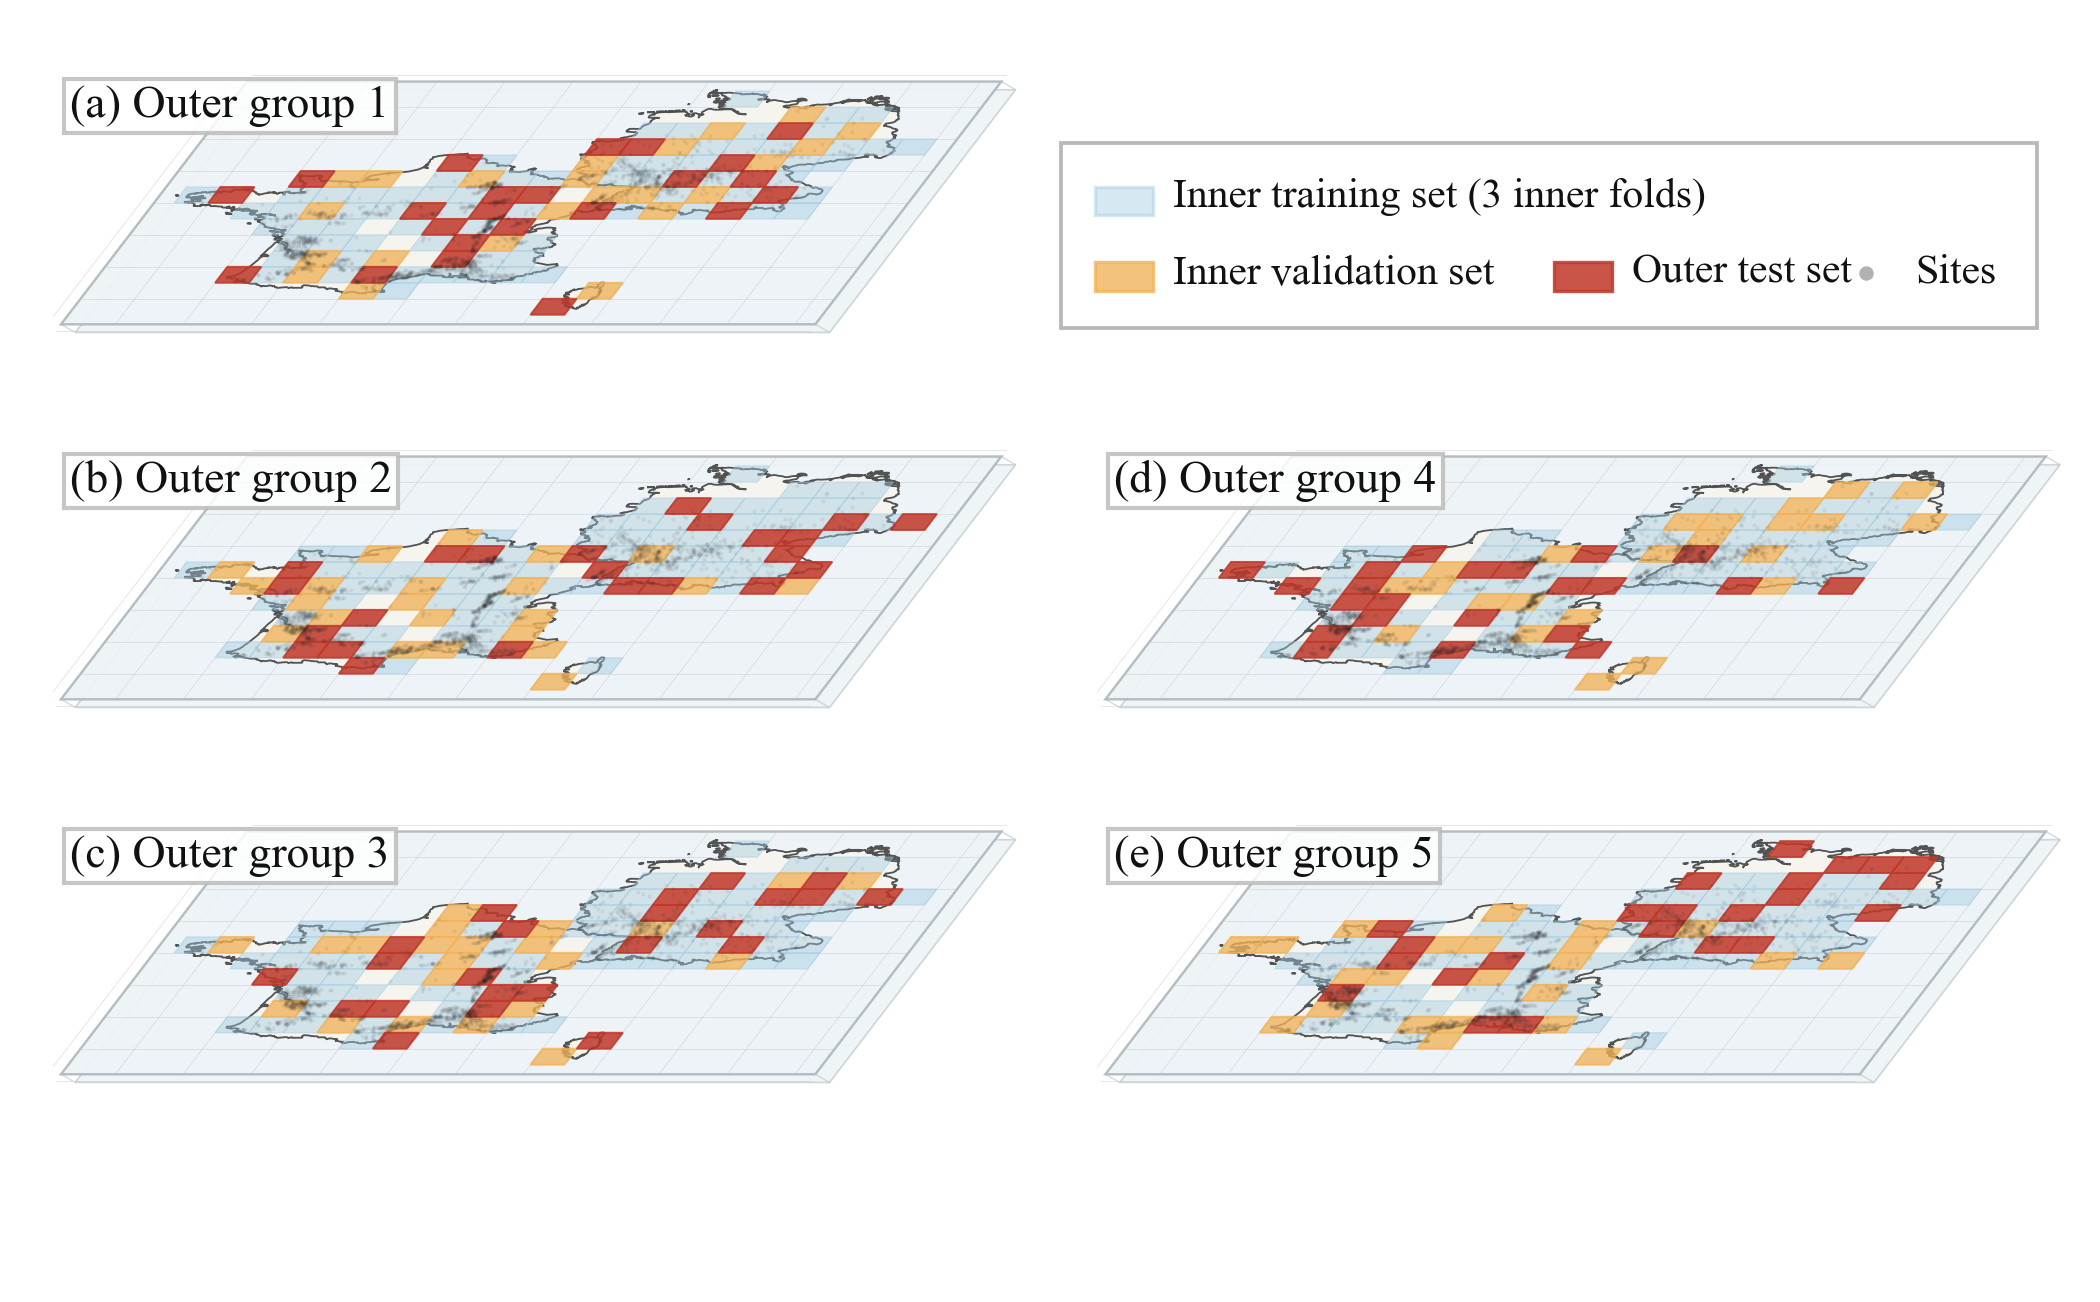
\includegraphics[width=\textwidth]{fig/spatial_validation/france_germany_era5_centered_1deg_nested_validation_layers.png}
\caption{Two-level blocked spatial validation design based on 1$^\circ$ ERA5-Land-centred spatial blocks. Each panel shows one outer spatial group held out as the outer test set and a representative split between the inner training set and inner validation set within the corresponding outer training set.}
\label{fig:nested_spatial_validation}
\end{figure}

\FloatBarrier

\subsubsection{Process-model calibration and selection}
\label{sec:process_model_calibration}

Process-model calibration followed the two-level spatial partitioning framework defined above. For each phenological stage and outer round, the outer test set was excluded from all calibration and selection steps. Within the corresponding outer training set, each candidate process-model structure was evaluated separately under the raw-temperature and elevation-adjusted-temperature branches. In each inner round, model parameters were estimated only from the inner training set: fixed-parameter benchmarks were used unchanged, GDD and GFV forcing thresholds were selected from 401 evenly spaced candidates spanning the accumulated forcing observed in the training data, and BRIN chilling and forcing thresholds were selected by a two-step grid search using 21 chilling and 201 forcing candidates. Root mean squared error (RMSE) was minimized in all calibrated cases. Candidates that did not reach their threshold within the available year were assigned a prediction one day beyond the end of that year for model-selection scoring, ensuring that failed predictions were retained as penalized errors rather than omitted.

Selection used only the four inner validation folds of the current outer training set. Candidate structures within each temperature branch were first screened to retain those whose mean penalized mean absolute error (MAE) was within one standard error of the minimum. The retained candidate with the lowest mean penalized RMSE was selected, with absolute pooled bias, between-fold MAE variability and worst-fold MAE applied sequentially as tie-breakers. The same rule was then used to compare the branch winners. When one model structure was selected in all five outer rounds but the preferred temperature branch differed, the structure was fixed and the branch selected within each outer round was retained. The selected process model was finally refitted on the full outer training set and used to predict the held-out outer test set.

\subsubsection{Residual learning and hybrid-model selection}

Residual learning used the two-level spatial partitioning framework described above. It also used the selected process-model configuration from Section~\ref{sec:process_model_calibration}. In each outer round, the selected process model was fitted and evaluated across the four inner rounds, producing out-of-fold process-model predictions for the inner validation sets. Residuals were calculated from Eq.~\ref{eq:residual_hybrid} as the difference between observed DOY and the corresponding out-of-fold process-model prediction. These residuals formed the machine-learning target within the current outer training set. Candidate machine-learning models used the same inner spatial folds for residual fitting and tuning, and predicted residual corrections for the inner validation sets.

The hybrid prediction was obtained by adding the machine-learning residual correction to the process-model prediction:

\begin{equation}
\widehat{DOY}_{\mathrm{hyb},i}
=
\widehat{DOY}_{\mathrm{proc},i}
+
\widehat{r}_{\mathrm{ML},i}
\label{eq:hybrid_prediction}
\end{equation}

Candidate hybrid systems, including the no-correction process-only baseline, were compared using hybrid DOY prediction errors on the inner validation sets. Missing predictor values were replaced by medians estimated from the current training subset. Predictors and residual targets were standardized within the training subset for Ridge and GAM models; the GAM used cubic spline bases with linear extrapolation. Preprocessing parameters were then applied unchanged to the corresponding validation or test subset. One residual-learning algorithm was fixed for each phenological stage by the lowest mean inner-validation RMSE across the five outer rounds, with MAE and absolute bias used as secondary ranking criteria. Within each outer round, hyperparameters for the fixed algorithm were selected by four-fold inner-validation RMSE before refitting on the complete outer training set. Stochastic learners used fixed fold-specific seeds derived from 20260805.

For final spatial evaluation, the selected ML model was fitted using residual records from the full outer training set and then applied to the held-out outer test set. The resulting outer-test predictions were used to evaluate whether residual correction improved generalization to spatially unseen records.

\subsection{Performance metrics and statistical summaries}
\label{sec:performance_metrics}

The following metrics were used to summarize prediction errors, paired model differences and fold-level variation. For evaluated record \(i\), \(y_i\) denotes the observed phenological day of year, \(\hat{y}_i\) denotes the predicted day of year, and \(n\) is the number of evaluated records.

\begin{align}
MAE &= \frac{1}{n}\sum_{i=1}^{n}\left|\hat{y}_i-y_i\right|
\label{eq:mae}\\
RMSE &= \sqrt{\frac{1}{n}\sum_{i=1}^{n}\left(\hat{y}_i-y_i\right)^2}
\label{eq:rmse}\\
Bias &= \frac{1}{n}\sum_{i=1}^{n}\left(\hat{y}_i-y_i\right)
\label{eq:bias}
\end{align}

MAE, RMSE and Bias summarize absolute, squared and signed prediction errors, respectively. Positive Bias indicates later predictions than observations, and negative Bias indicates earlier predictions.

For any metric \(M\), paired model differences were defined as:

\begin{equation}
\Delta M = M_A - M_B
\label{eq:metric_difference}
\end{equation}

where \(A\) denotes the tested model or branch and \(B\) denotes the reference model or branch. Negative \(\Delta M\) values indicate lower error for \(A\). The relative gain was calculated as:

\begin{equation}
Gain_M = \frac{M_B-M_A}{M_B}\times100\%
\label{eq:metric_gain}
\end{equation}

For fold-specific metric \(M_k\), the fold mean and standard error were:

\begin{equation}
\overline{M}=\frac{1}{K}\sum_{k=1}^{K}M_k,\qquad
SE=\frac{sd(M_k)}{\sqrt{K}},\qquad K=5
\label{eq:fold_summary}
\end{equation}

Worst-fold performance was defined as \(\max_k M_k\) for fold-specific MAE or RMSE.

\endgroup

\section{Results}

\begingroup
\setlength{\parindent}{0pt}
\setlength{\parskip}{0.5\baselineskip}

\subsection{Spatial pattern and magnitude of terrain-temperature correction}

Terrain-based temperature correction showed a clear spatial pattern across the French and German phenology sites (Fig.~\ref{fig:terrain_temperature_correction}). Correction magnitudes were low to moderate over most of the study region, whereas larger corrections occurred where vineyards were located in more topographically complex areas. At the country scale, Fig.~\ref{fig:terrain_temperature_correction} further shows that low-magnitude corrections accounted for a larger proportion of the French records, while medium- to high-magnitude corrections accounted for a larger proportion of the German records.

\begin{figure}[!htb]
\centering
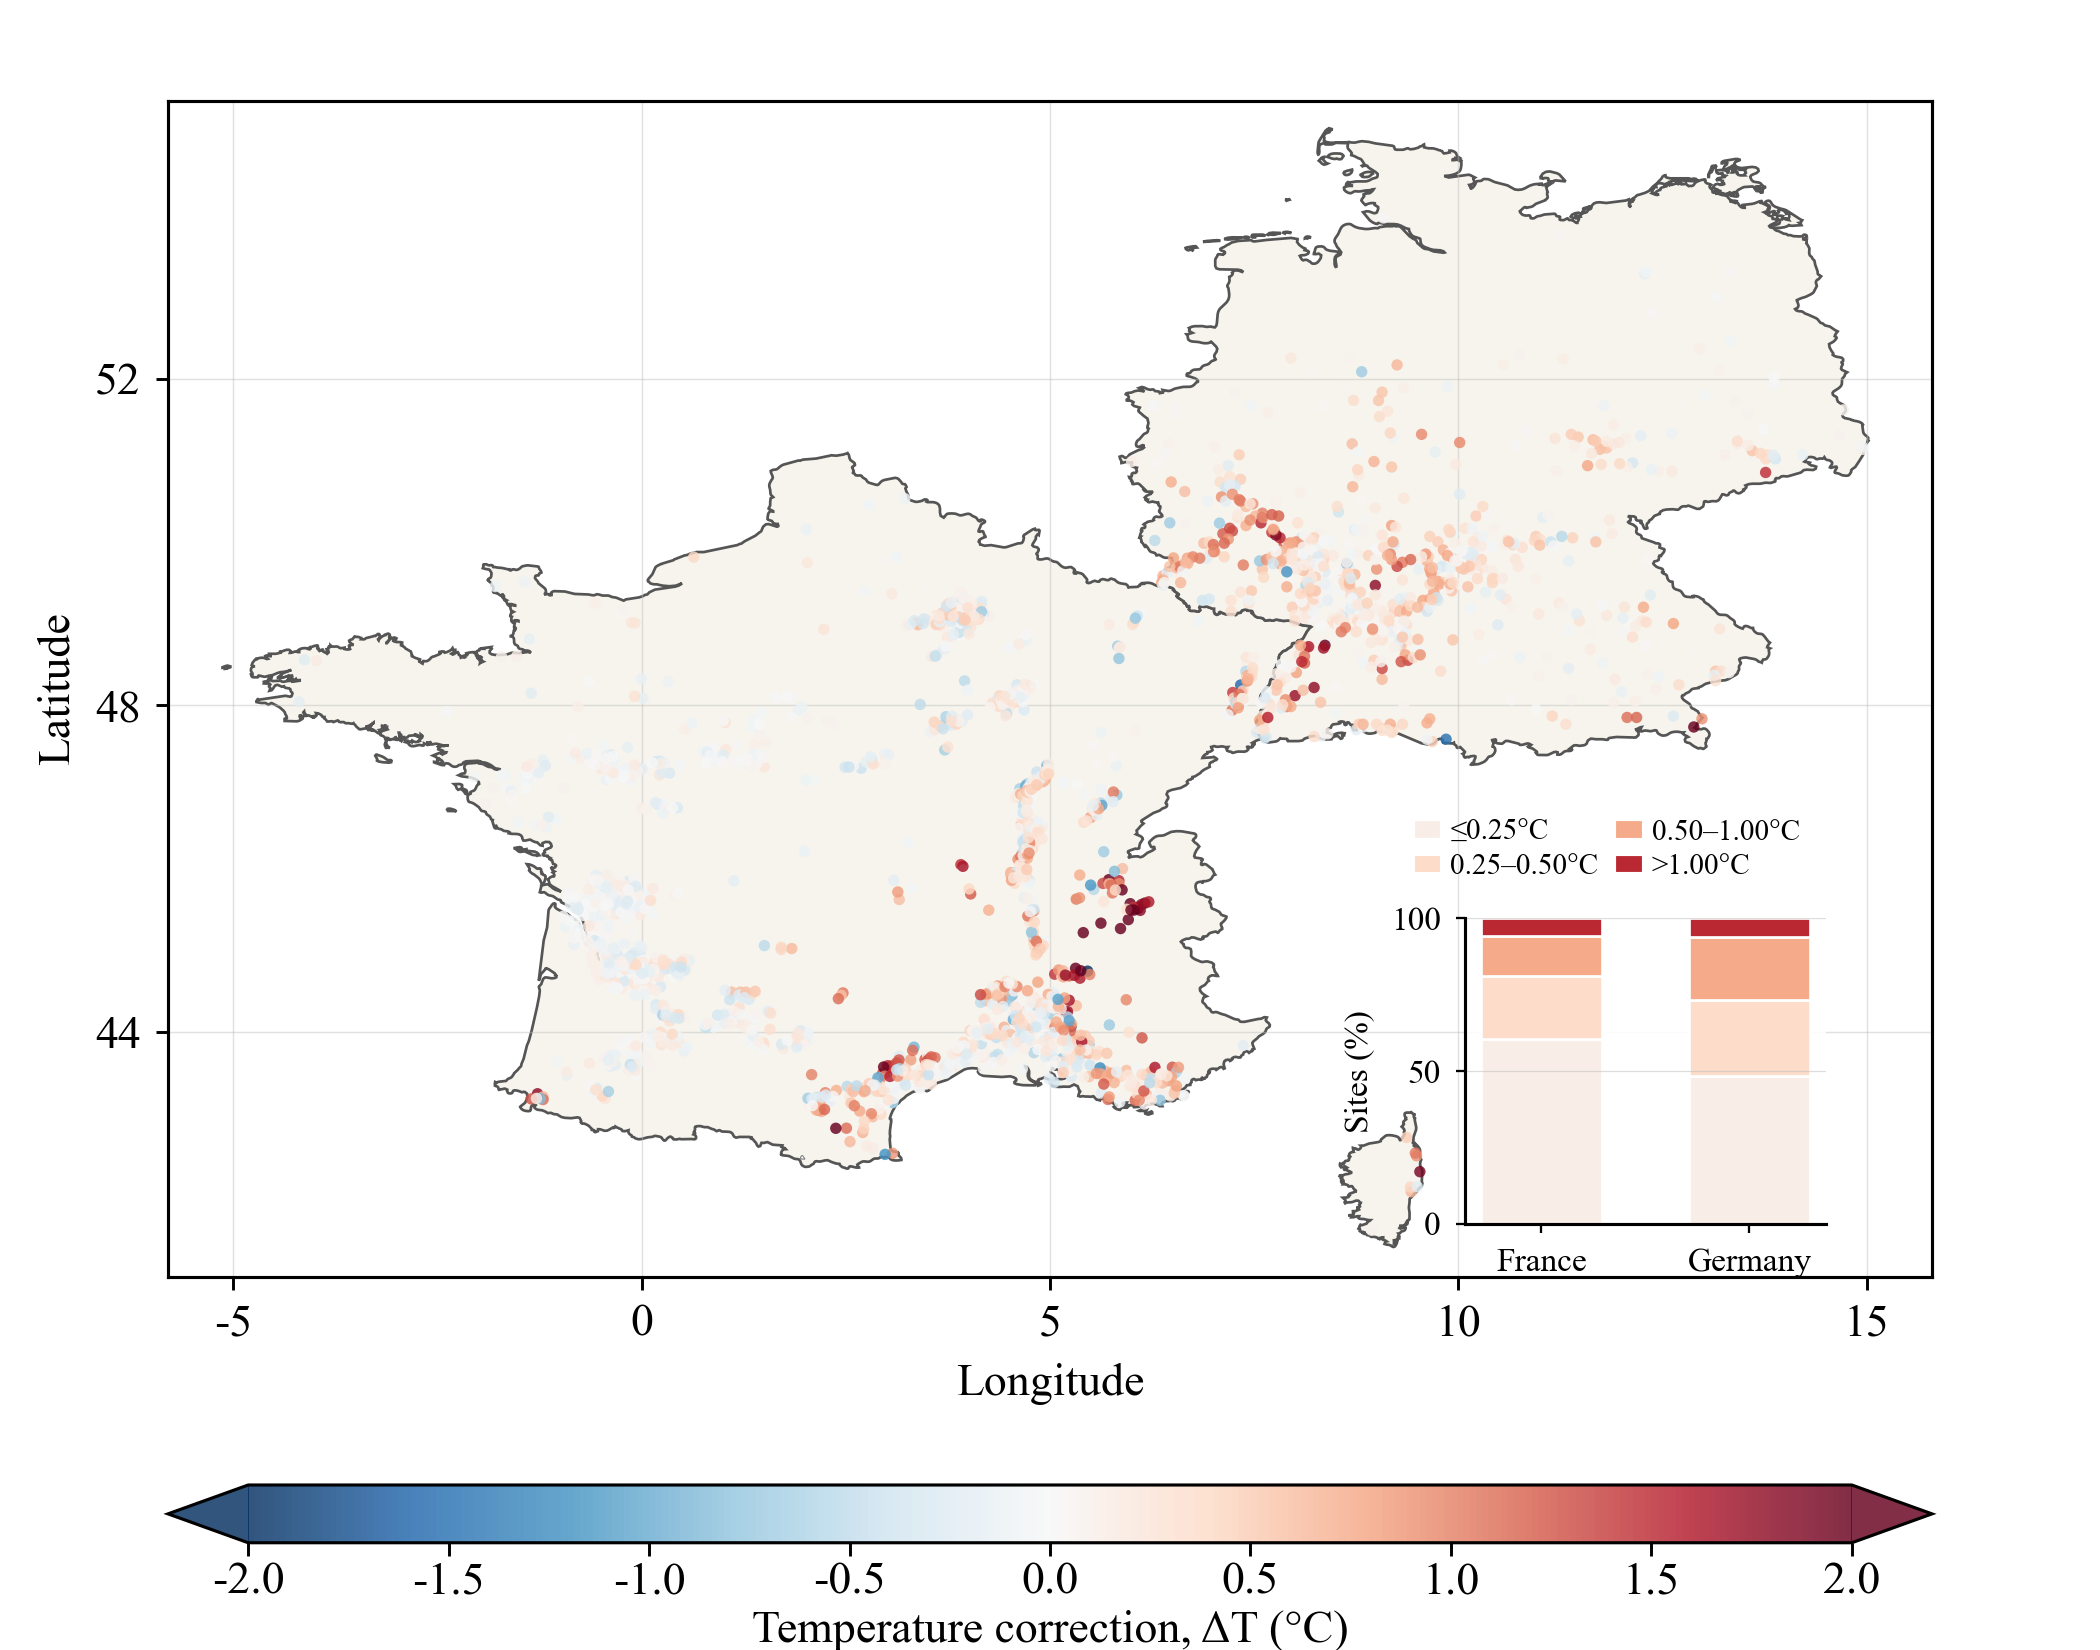
\includegraphics[width=\textwidth]{fig/results_figure/terrain_temperature_correction_strength.png}
\caption{Spatial distribution and magnitude of terrain-based temperature correction across the French and German grapevine phenology sites. The inset summarizes the country-level proportional distribution of correction magnitudes.}
\label{fig:terrain_temperature_correction}
\end{figure}

\FloatBarrier
\subsection{Process-model performance and terrain-temperature effects}

Process-model performance varied markedly among phenological stages and model structures (Fig.~\ref{fig:process_model_temperature}). Based on RMSE, the best-performing process models for BBCH07, BBCH65, BBCH81 and BBCH89 were BRIN, GFV, GFV and the stage-to-stage GDD10 model, respectively. For the temperature-forcing branch, BBCH07 retained the branch selected within each outer round, whereas BBCH65, BBCH81 and BBCH89 selected the terrain-adjusted temperature branch.

The selected process-model baselines reached MAE/RMSE values of 6.8/9.6~d for BBCH07, 5.7/8.2~d for BBCH65, 12.4/15.5~d for BBCH81, and 27.8/30.5~d for BBCH89 (Fig.~\ref{fig:process_model_temperature}a,b). Flowering showed the highest prediction accuracy, whereas maturity/harvest had markedly larger errors. Observed--predicted comparisons further showed that BBCH65 strict spatial outer-fold predictions were densely distributed near the 1:1 reference line, with small model bias. BBCH07 and BBCH81 showed broader point dispersion, whereas BBCH89 exhibited a pronounced overall negative bias of -27.0~d (Fig.~\ref{fig:selected_process_observed_predicted}).

Terrain-adjusted temperature produced only small changes in the selected budburst and flowering models, but larger improvements for later phenological stages (Fig.~\ref{fig:process_model_temperature}c,d). The RMSE change was -0.06~d for BBCH07 and -0.14~d for BBCH65, compared with -1.28~d for BBCH81 and -2.17~d for BBCH89. Within the same phenological stage, the magnitude of the temperature-adjustment effect also varied among process-model structures.

\begin{figure}[!htbp]
\centering
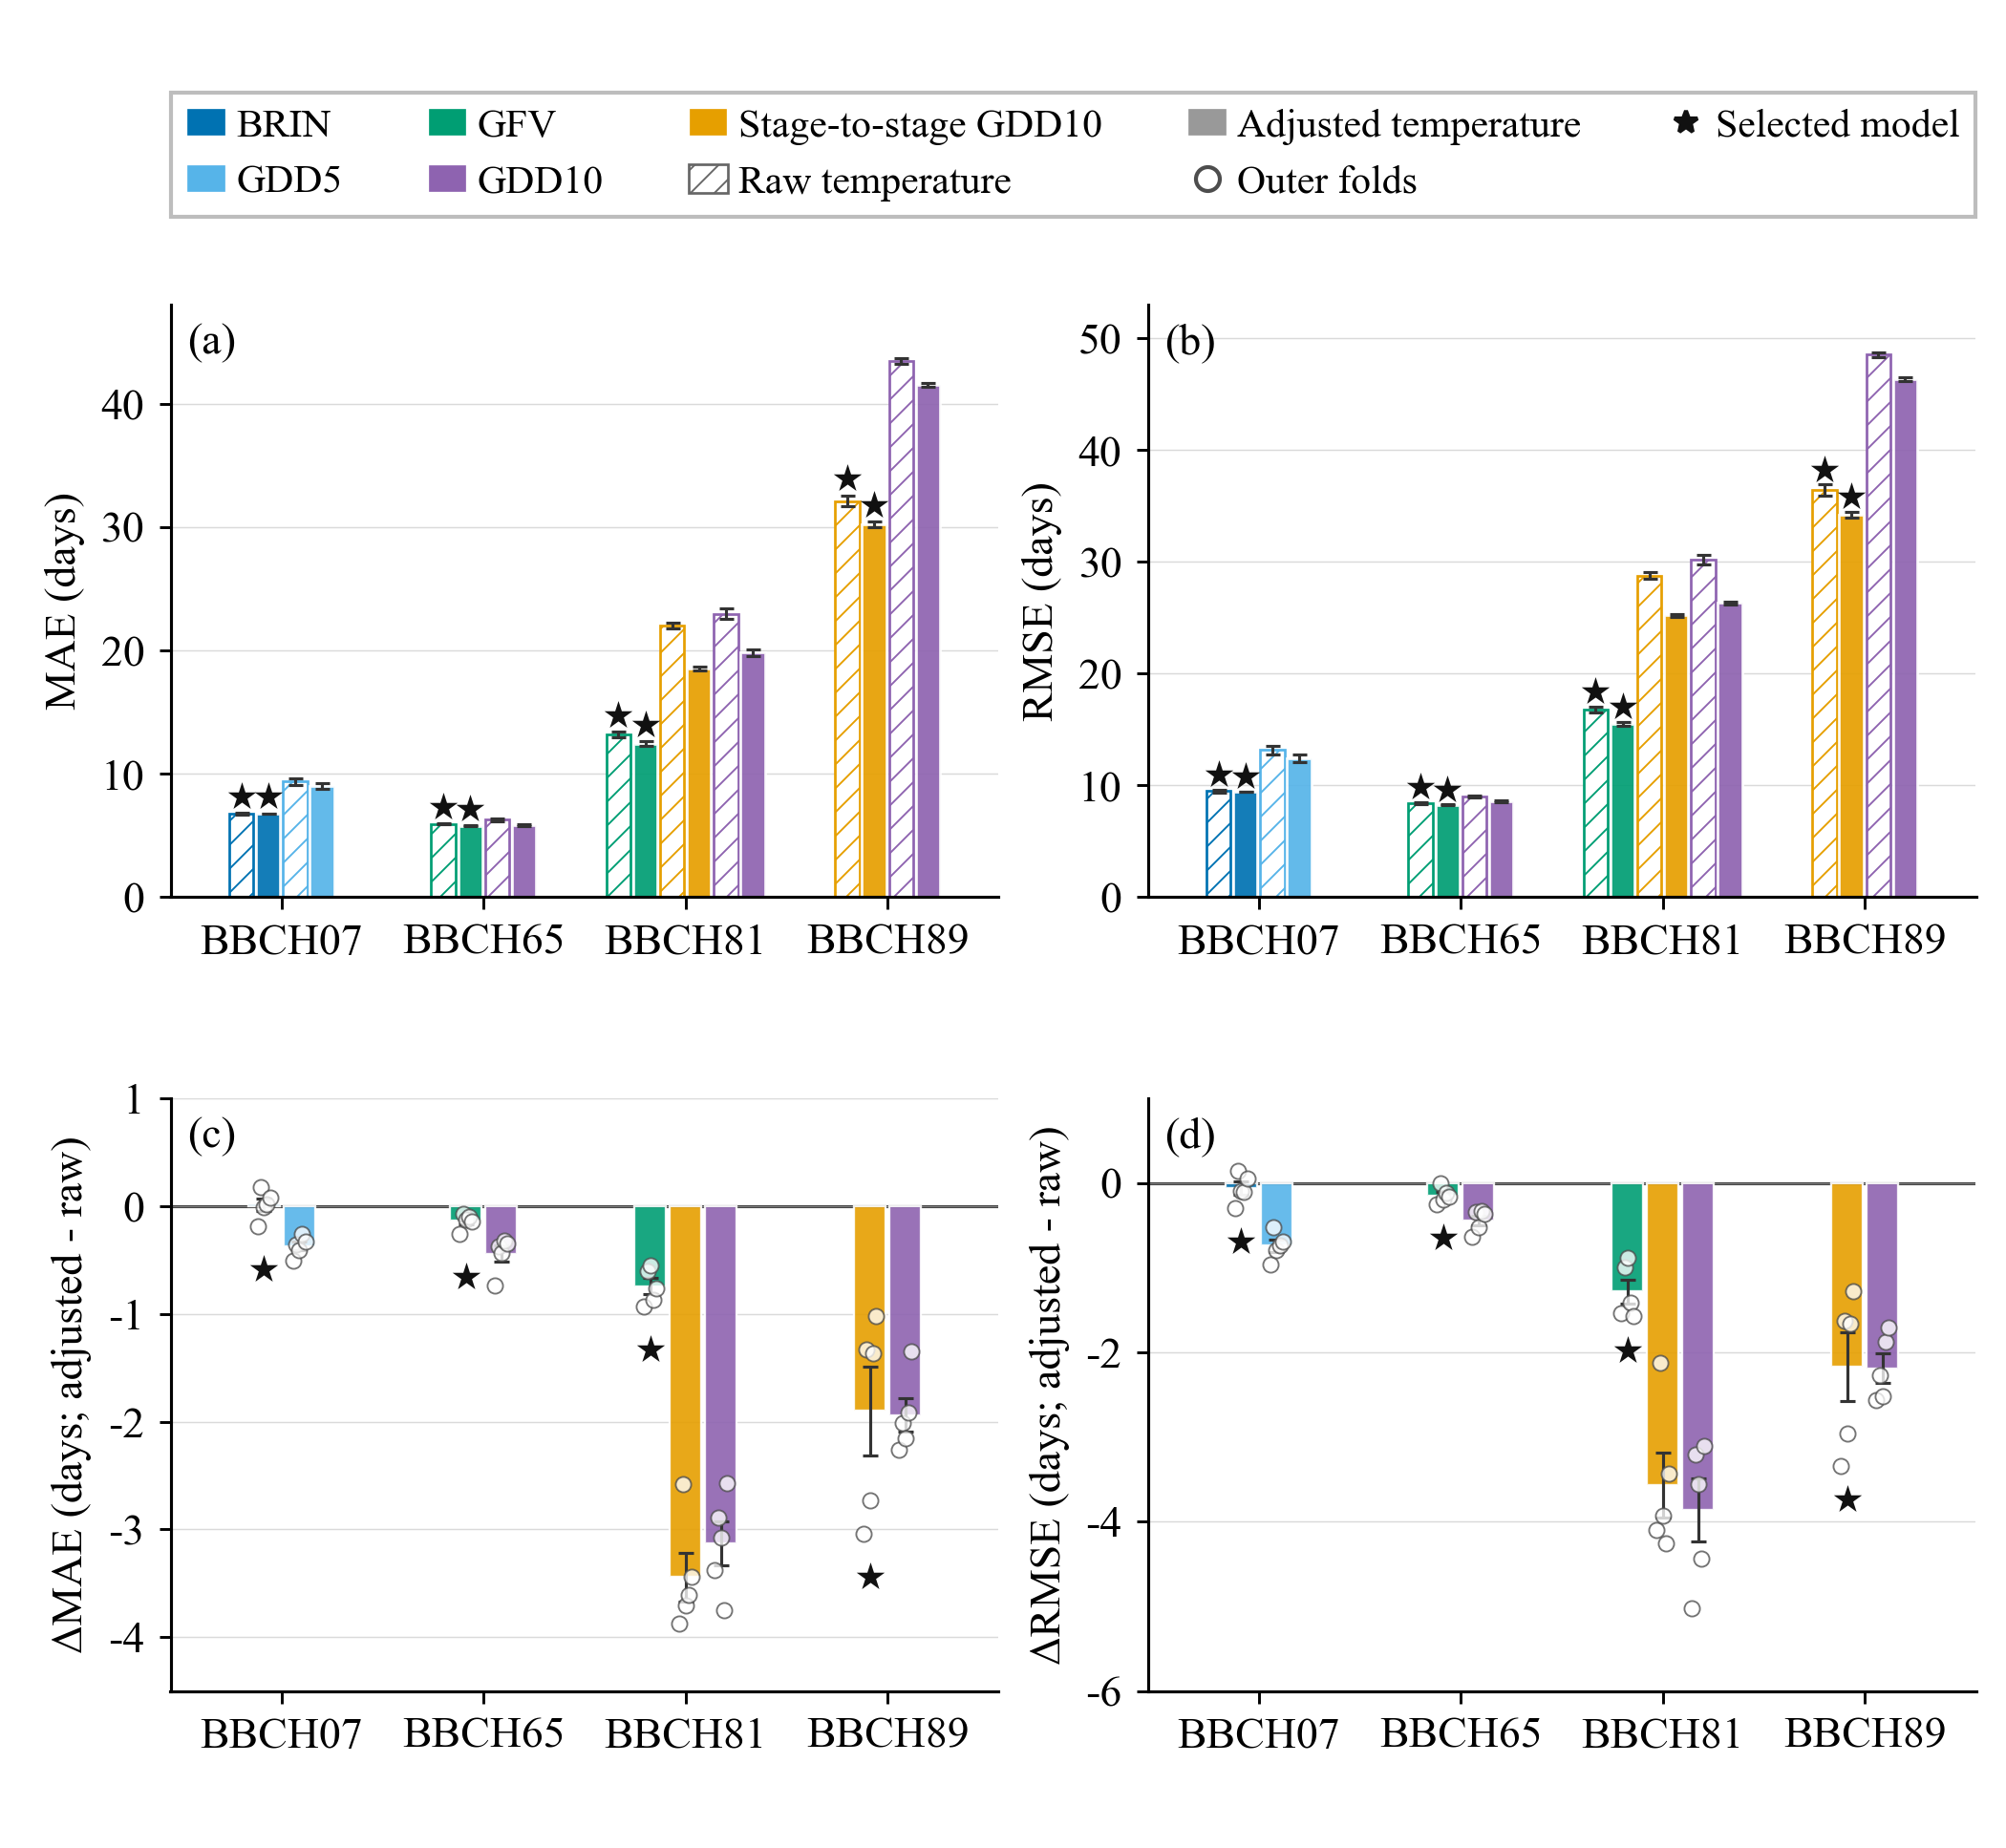
\includegraphics[width=\textwidth]{fig/results_figure/raw_vs_adjusted_process_model_combined.png}
\caption{Simulation performance of candidate process models driven by raw and terrain-adjusted temperatures (a--b). Bars show means across outer rounds, and open circles show individual outer-test estimates. Panels (c--d) show error differences between terrain-adjusted and raw temperature inputs. Negative values indicate reduced process-model prediction error after terrain adjustment.}
\label{fig:process_model_temperature}
\end{figure}

\begin{figure}[!htbp]
\centering
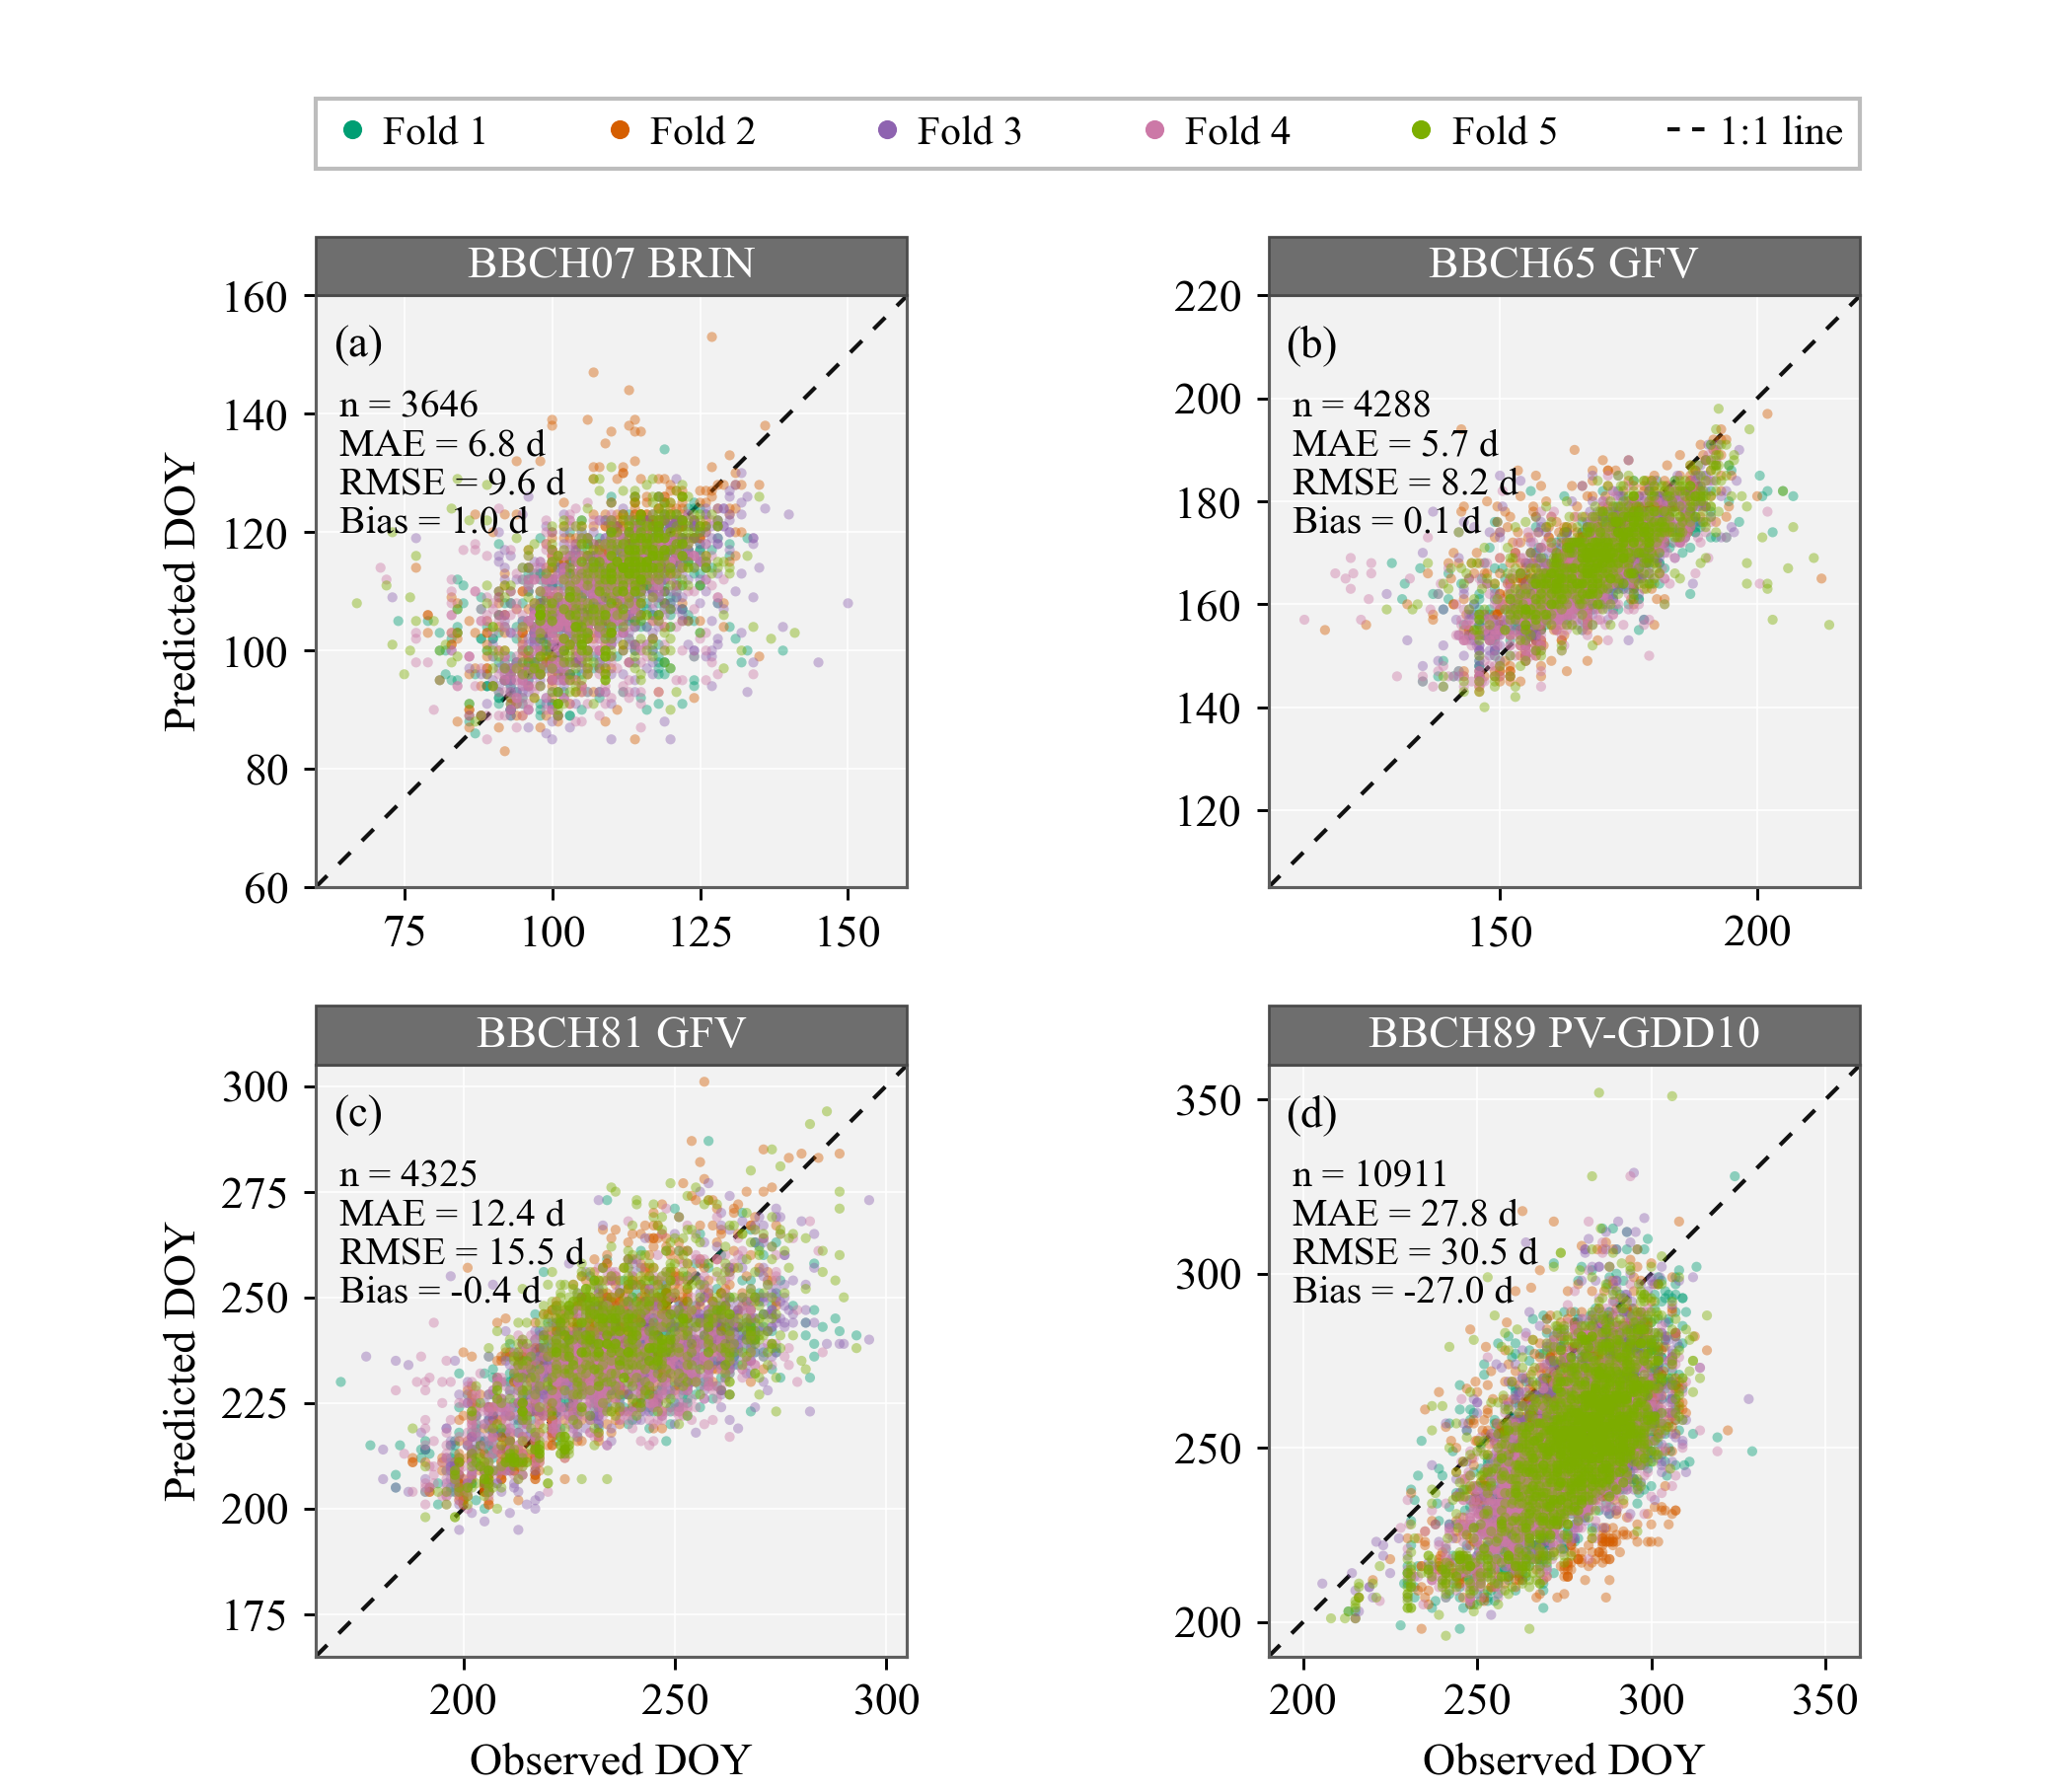
\includegraphics[width=\textwidth]{fig/results_figure/selected_process_model_observed_predicted.png}
\caption{Observed and predicted phenological day of year for the selected process-model baseline at each stage. Points are outer-test predictions, and colors denote outer spatial groups.}
\label{fig:selected_process_observed_predicted}
\end{figure}

\FloatBarrier
\subsection{Machine-learning model selection and hybrid-model accuracy gains}

Hybrid models with machine-learning residual correction improved upon the selected process-model baseline in all four phenological stages (Fig.~\ref{fig:residual_ml_candidates}). Based on RMSE, the fixed hybrid combinations were Ridge for BBCH07, RF for BBCH65, Ridge for BBCH81, and RF for BBCH89 (Fig.~\ref{fig:residual_ml_candidates}a,b). From BBCH07 to BBCH81, candidate machine-learning models showed similar and modest improvements, whereas the improvement was much larger for BBCH89.

RMSE decreased from 9.6 to 8.3~d for BBCH07, from 8.2 to 7.7~d for BBCH65, from 15.5 to 14.6~d for BBCH81, and from 30.5 to 10.6~d for BBCH89. These reductions corresponded to RMSE decreases of 12.7\%, 6.0\%, 5.8\%, and 65.4\%, respectively. MAE showed the same direction of change as RMSE, with the largest absolute reduction again observed for BBCH89 (Fig.~\ref{fig:residual_ml_candidates}c,d).

Observed--predicted comparisons of the fixed hybrid models showed near-zero aggregate bias in all four phenological stages (Fig.~\ref{fig:selected_hybrid_observed_predicted}). BBCH65 remained densely clustered around the 1:1 reference line. BBCH07 and BBCH81 still showed broader point dispersion, but their aggregate biases were reduced relative to the process-only models. For BBCH89, the fixed hybrid model substantially reduced the negative bias observed in the process-only model, changing the aggregate bias from -27.0 to -0.1~d.

\begin{figure}[!htbp]
\centering
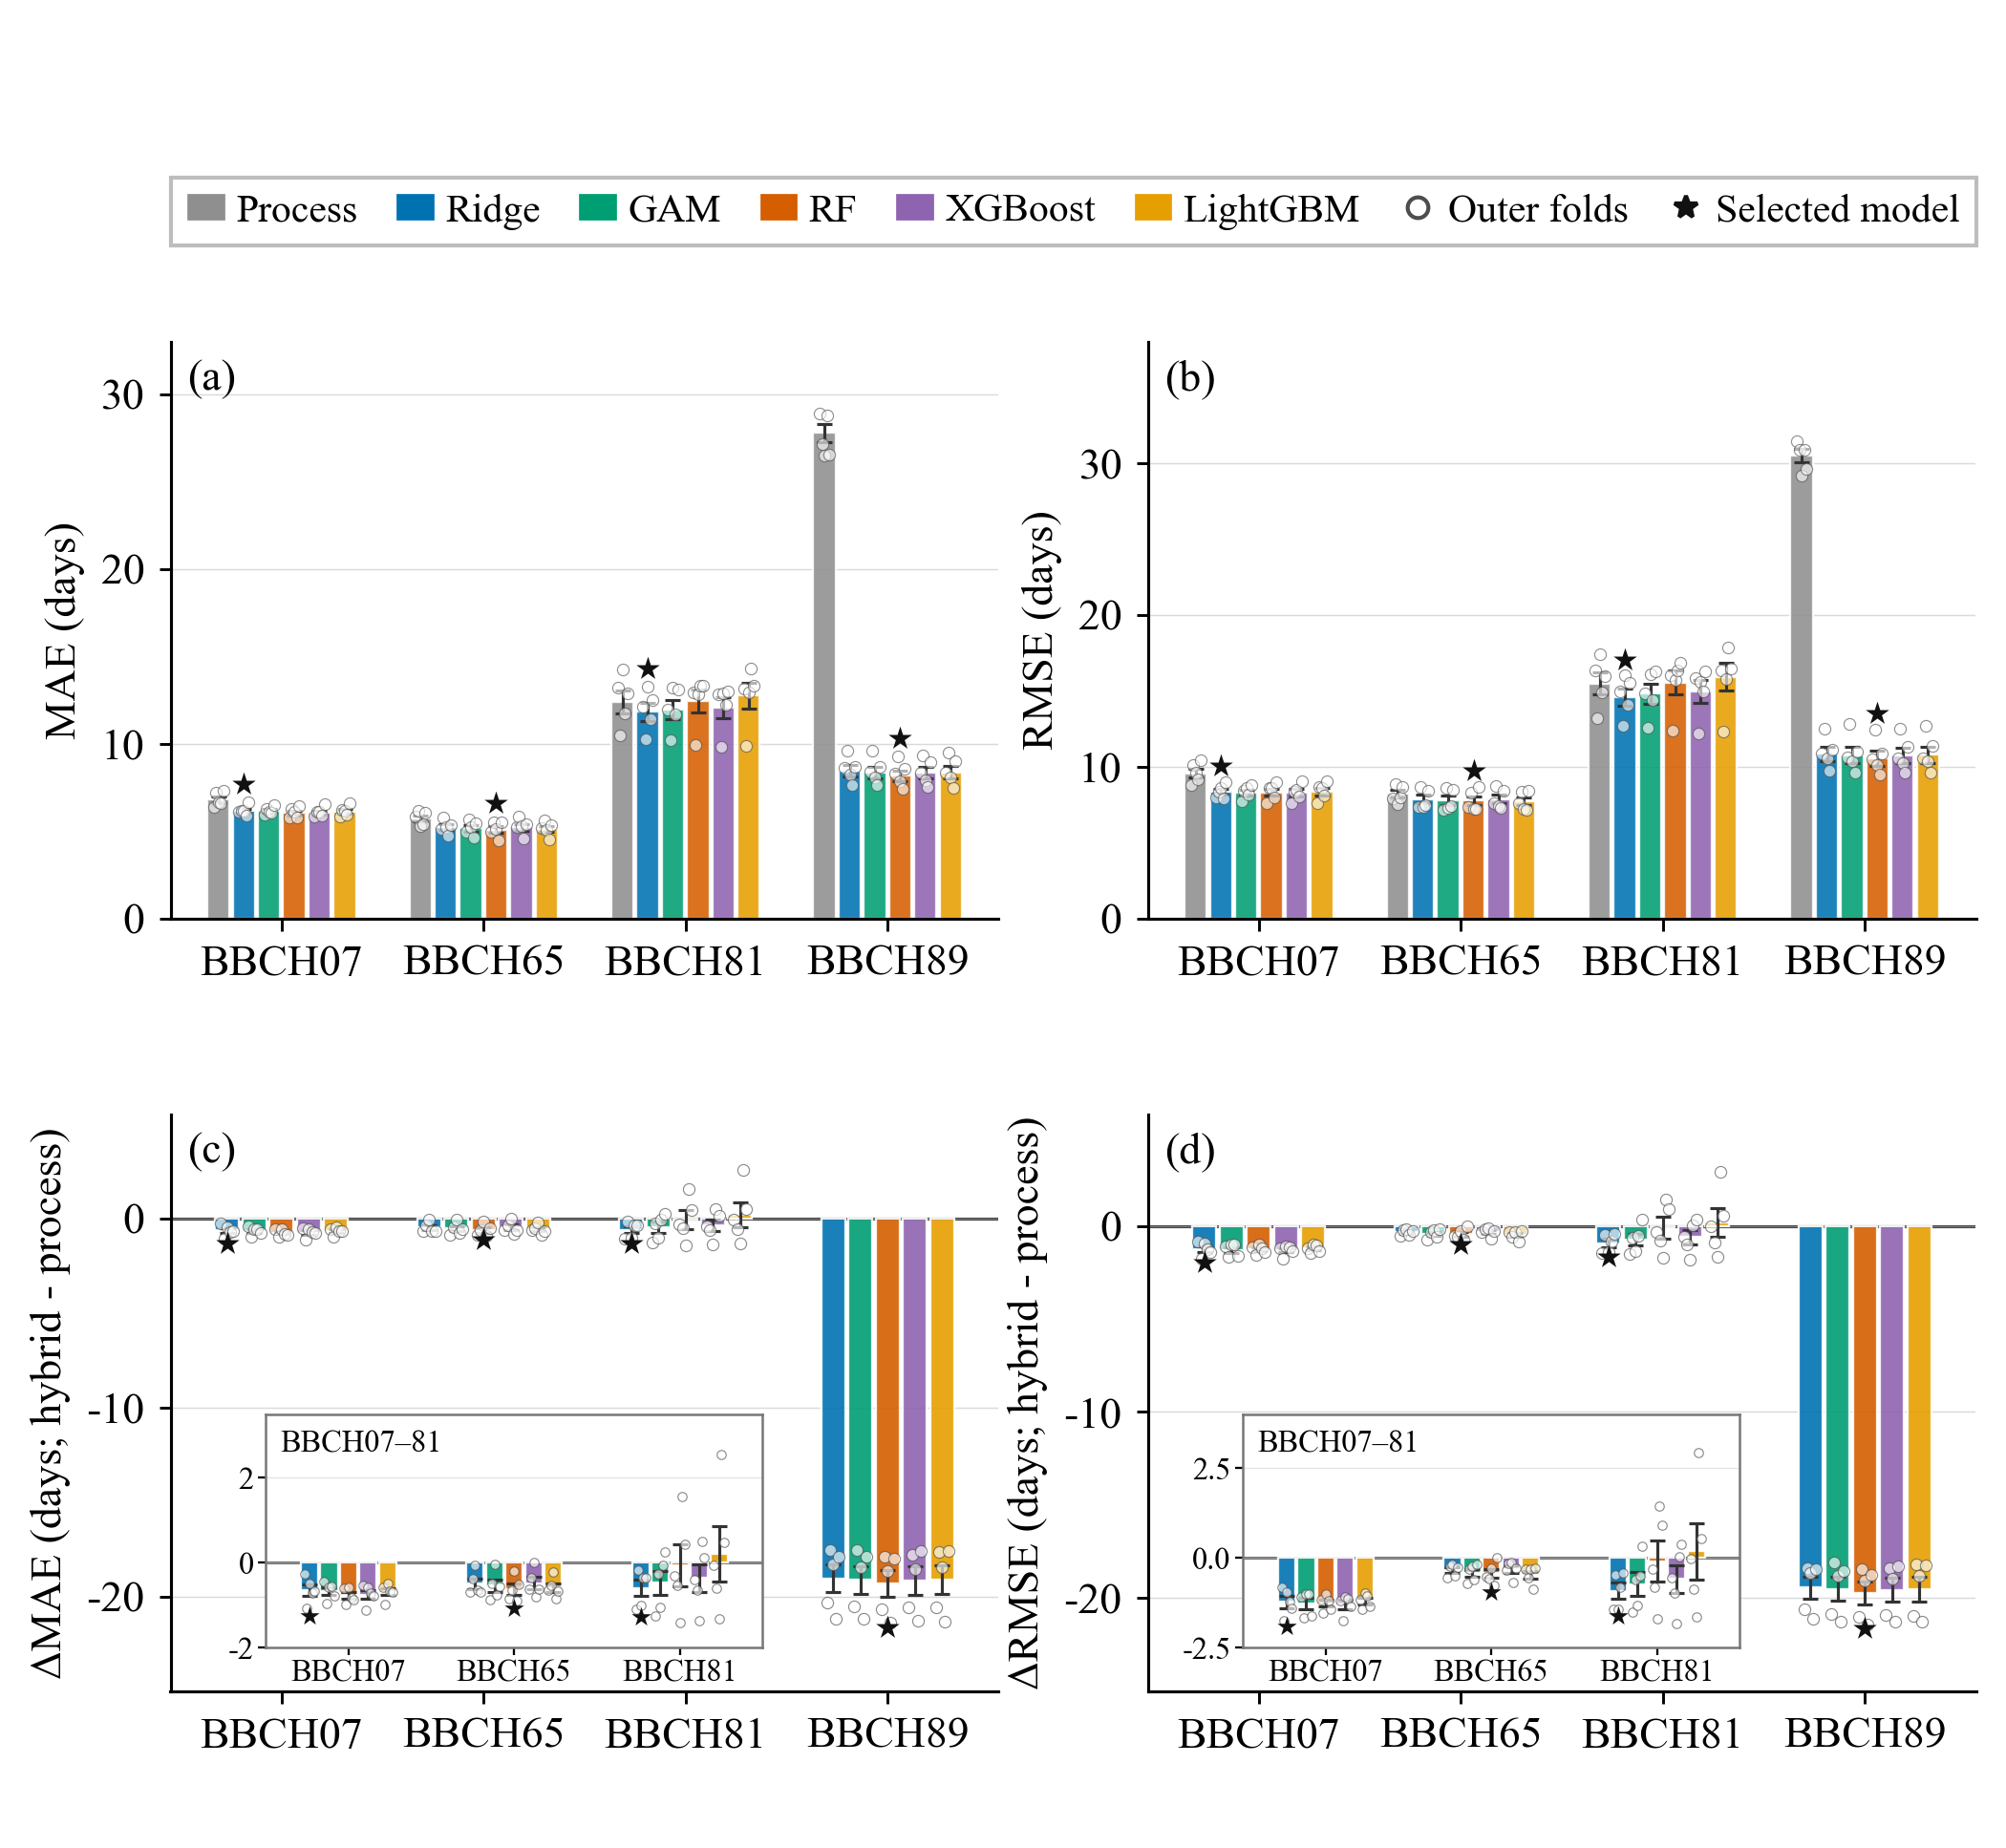
\includegraphics[width=\textwidth]{fig/results_figure/residual_ml_candidate_model_performance.png}
\caption{Residual-learning performance of machine-learning models for the main phenological stages (a--b). Open circles show individual outer-test estimates from the five outer rounds. Error changes of hybrid models relative to the process-only models are shown in (c--d). Negative values indicate reduced prediction error after residual correction.}
\label{fig:residual_ml_candidates}
\end{figure}

\begin{figure}[!htbp]
\centering
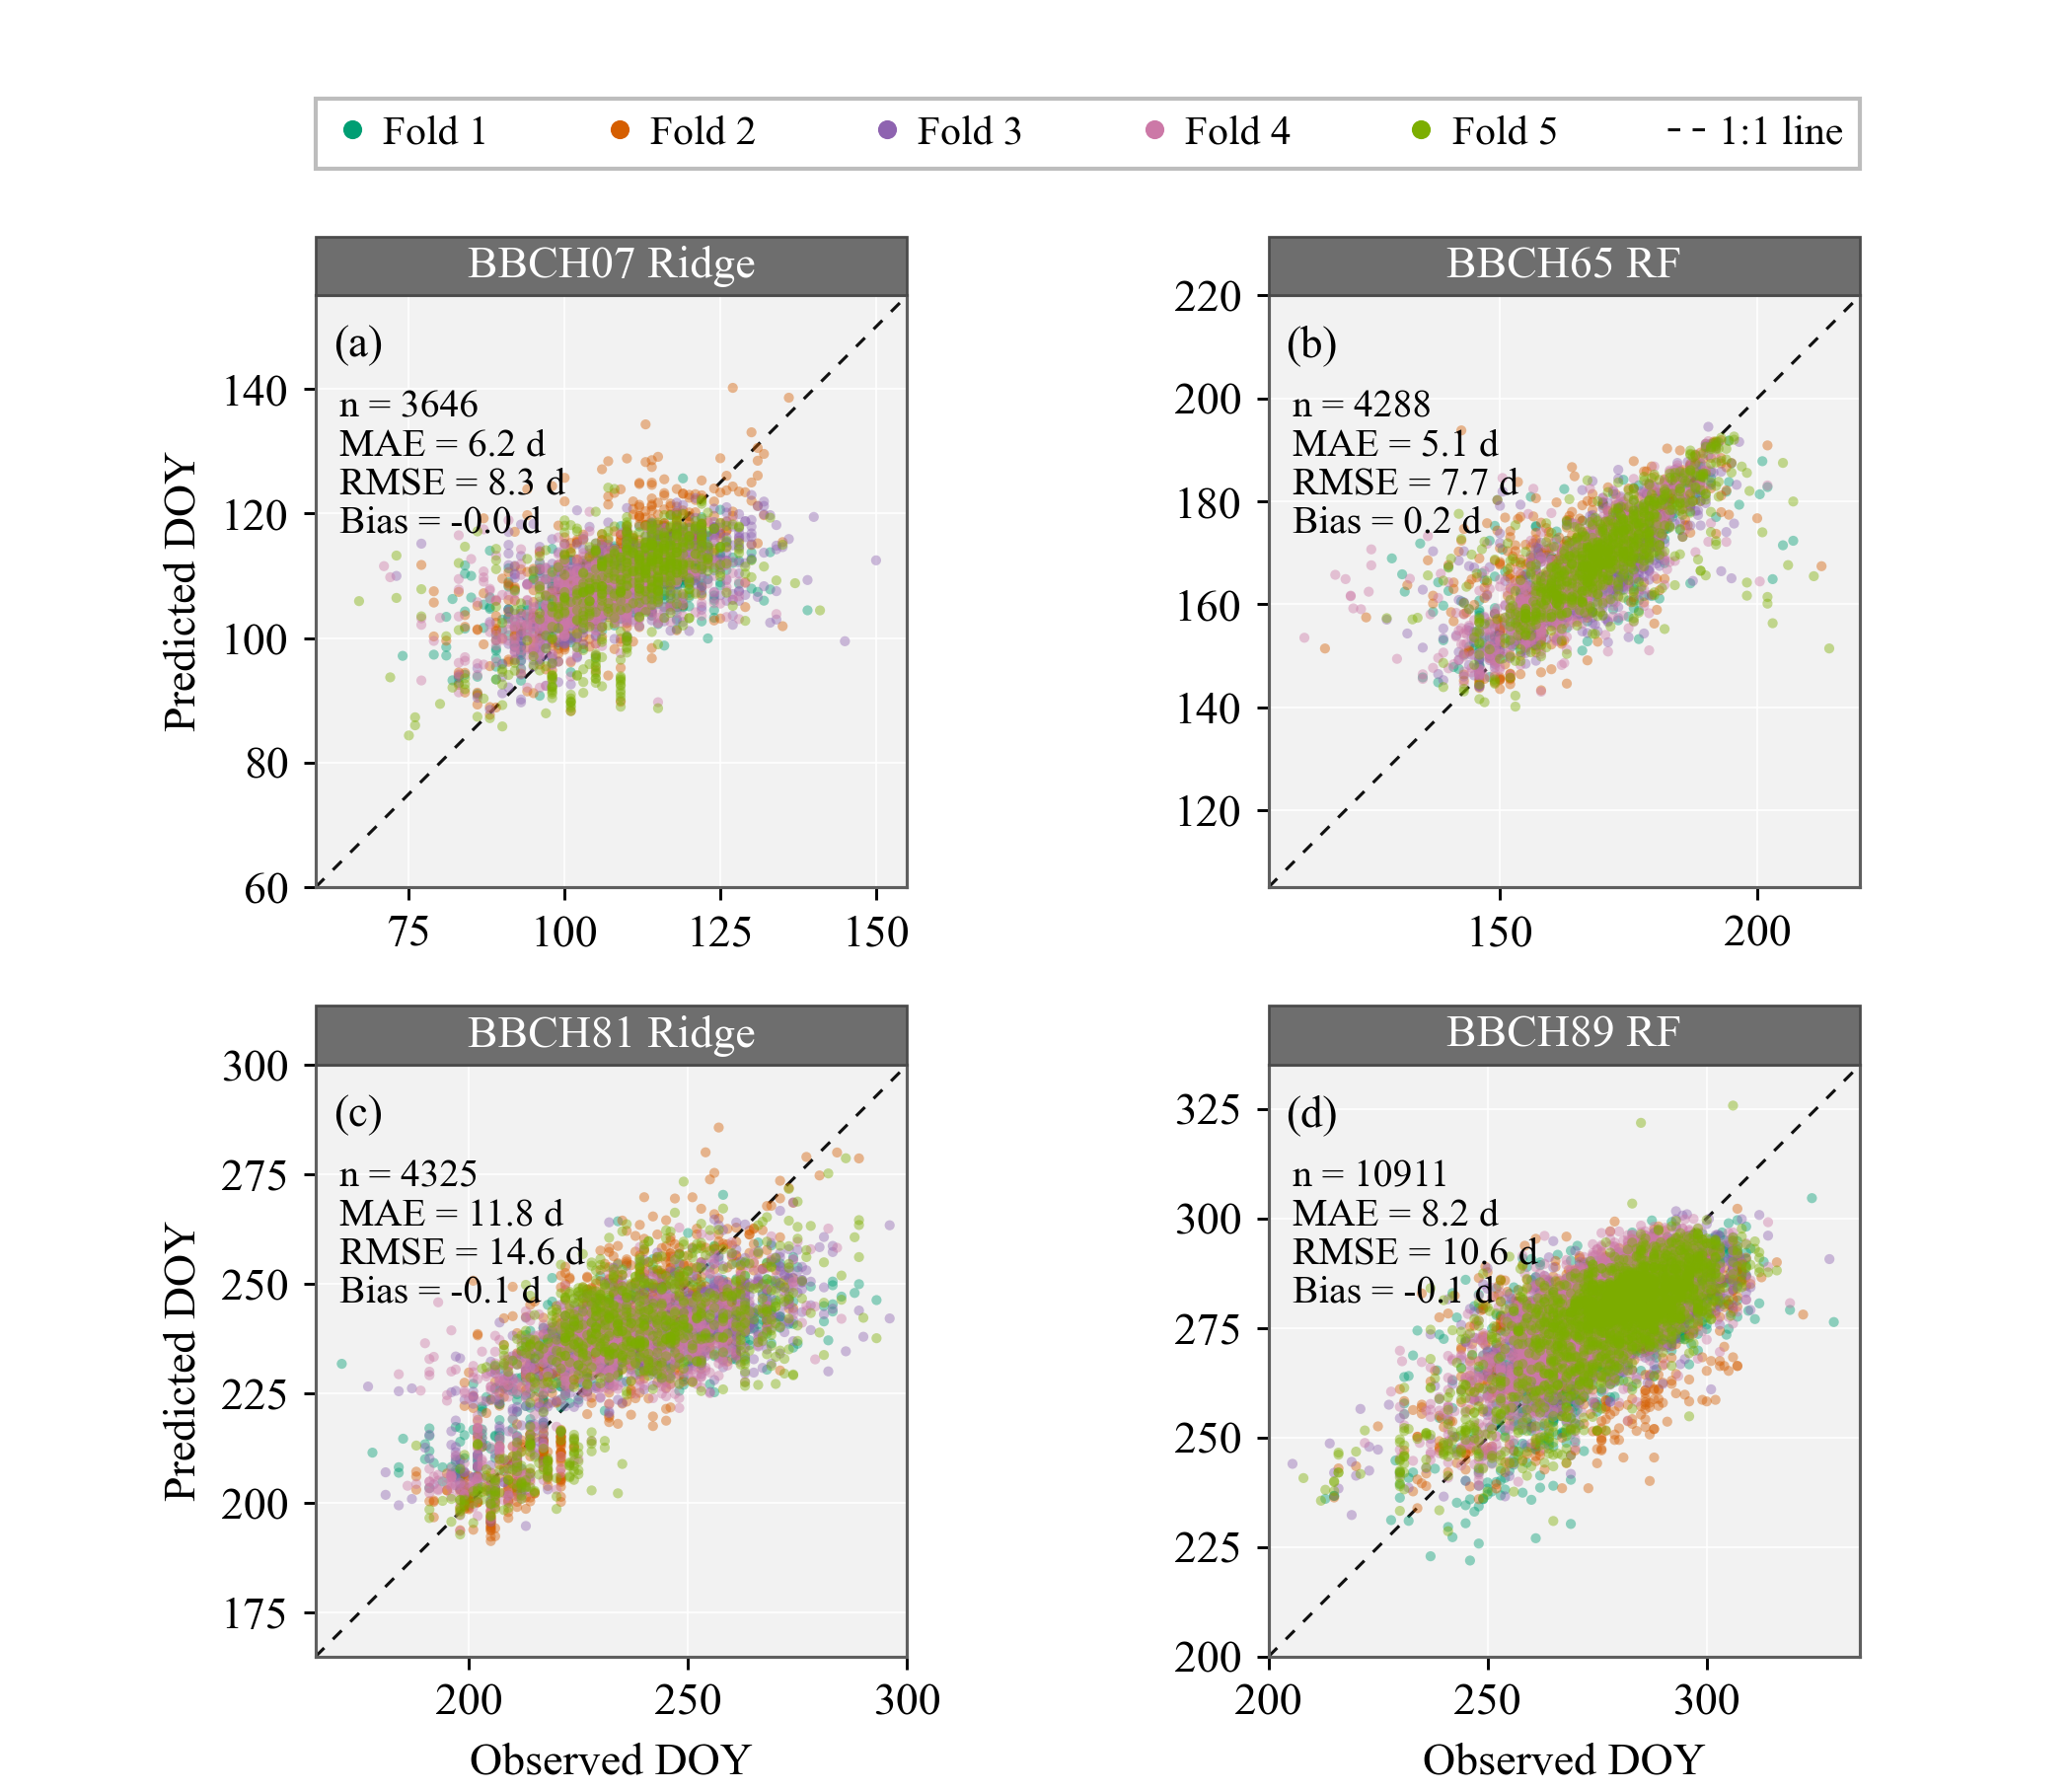
\includegraphics[width=\textwidth]{fig/results_figure/selected_hybrid_model_observed_predicted.png}
\caption{Observed and predicted phenological day of year for the fixed hybrid model at each stage. Points are outer-test predictions, and colors denote outer spatial groups.}
\label{fig:selected_hybrid_observed_predicted}
\end{figure}

\FloatBarrier
\subsection{Spatial robustness of hybrid-model gains}

The accuracy gains from the hybrid models remained stable across the five outer rounds (Fig.~\ref{fig:spatial_generalization_gain}). MAE and RMSE decreased in every held-out outer test set for each phenological stage. Although the magnitude of improvement differed among stages, no outer round showed a reversal in which the fixed hybrid model performed worse than the corresponding process-only model.

Residual correction also improved the worst outer-round performance. The maximum outer-test RMSE across outer rounds decreased from 10.4 to 9.0~d for BBCH07, from 8.9 to 8.5~d for BBCH65, from 17.4 to 16.0~d for BBCH81, and from 31.5 to 12.4~d for BBCH89. The mean outer-round RMSE differences were -1.2, -0.5, -0.9, and -19.7~d for BBCH07, BBCH65, BBCH81, and BBCH89, respectively.

\begin{figure}[!htbp]
\centering
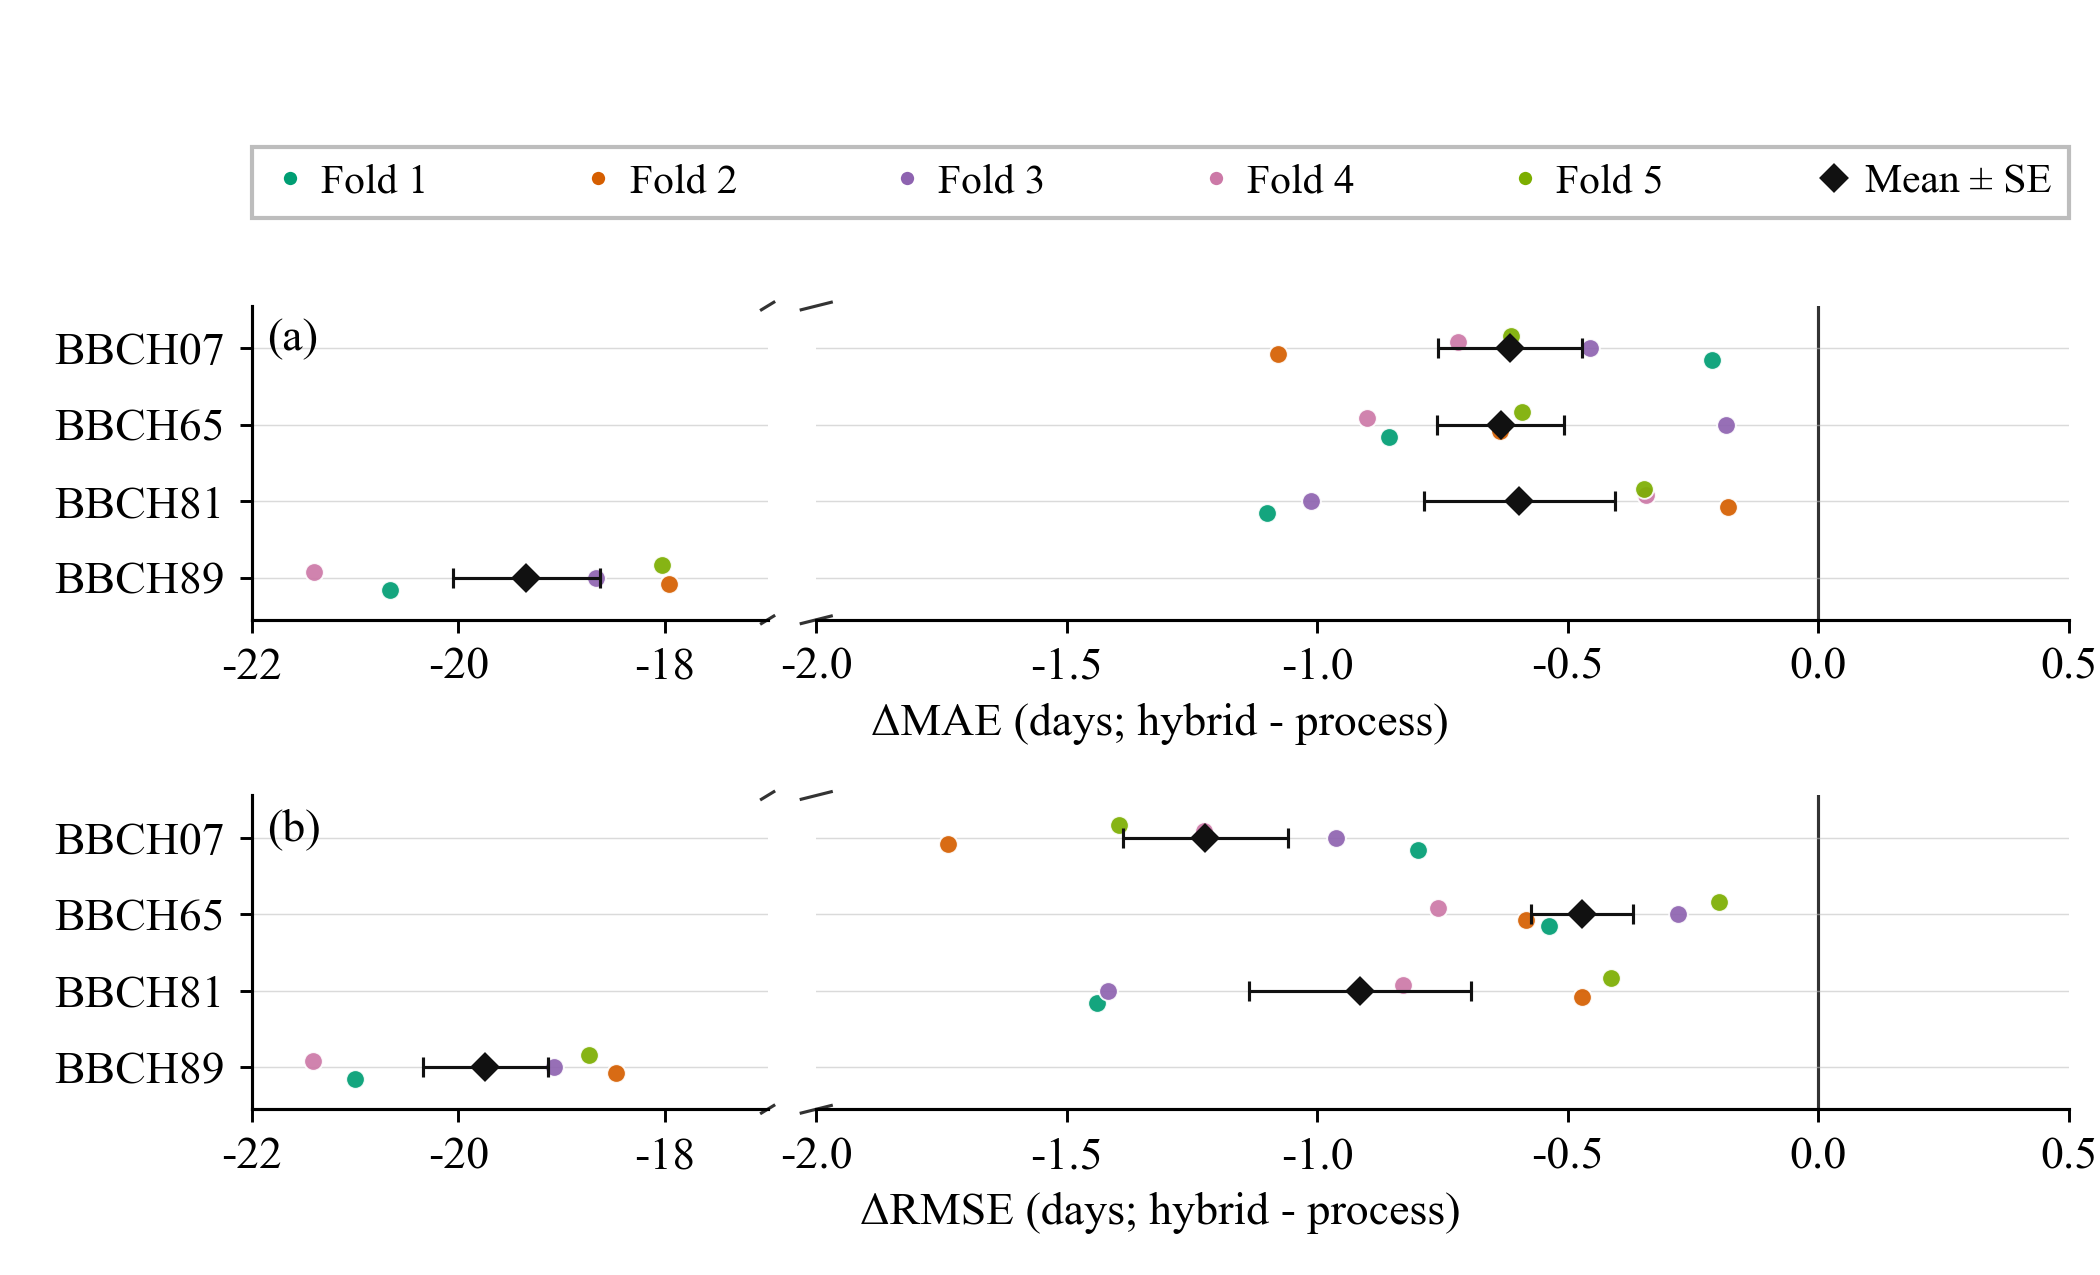
\includegraphics[width=\textwidth]{fig/results_figure/spatial_generalization_foldwise_gain_forest.png}
\caption{Accuracy gains of the best hybrid models across the five outer rounds. Delta values are hybrid-model error minus process-model error. Negative values indicate lower error than the selected process model. The x-axis is shown with a broken scale.}
\label{fig:spatial_generalization_gain}
\end{figure}

\FloatBarrier
\subsection{Mechanism-group and feature-level residual interpretability}

Mechanism-group ablation showed that the residual information retained by the fixed hybrid models followed a stage-dependent pattern (Fig.~\ref{fig:mechanism_group_ablation}). Removing the process-state group caused the largest RMSE increase for BBCH07 (+0.87~d) and BBCH89 (+0.18~d). For BBCH65, the largest increase was associated with temperature-structure variables (+0.19~d). For BBCH81, the terrain/spatial group had the largest contribution (+0.42~d), followed by process-state and process-timing variables.

The remaining groups had smaller and less uniform effects. Water/drought variables increased RMSE when removed from BBCH65 and BBCH89, but produced little change for BBCH81. Radiation variables contributed weakly but positively in BBCH07, BBCH65 and BBCH89. Terrain/spatial removal did not increase RMSE in every stage, showing that group-level contributions were not transferable as a single common ranking across the four phenological events.

Feature-level SHAP patterns confirmed that the dominant residual predictors differed among stages (Fig.~\ref{fig:shap_residual_beeswarm}).

In BBCH07, process-predicted DOY was the strongest feature, followed by pre-BBCH07 GDD5 accumulation rate, latitude, elevation, shortwave radiation, frost intensity and preseason chill. In BBCH65, elevation and BBCH07--65 GDD10 accumulation rate ranked highest, followed by radiation, diurnal temperature range and northness. In BBCH81, predicted BBCH65--81 interval length, longitude and latitude dominated the SHAP ranking, with additional contributions from heat intensity, local elevation variability and pre-veraison climatic water deficit. In BBCH89, pre-BBCH89 GDD10 rate and process-predicted DOY were the leading features, followed by elevation, radiation and VPD-related variables.

\begin{figure}[!htbp]
\centering
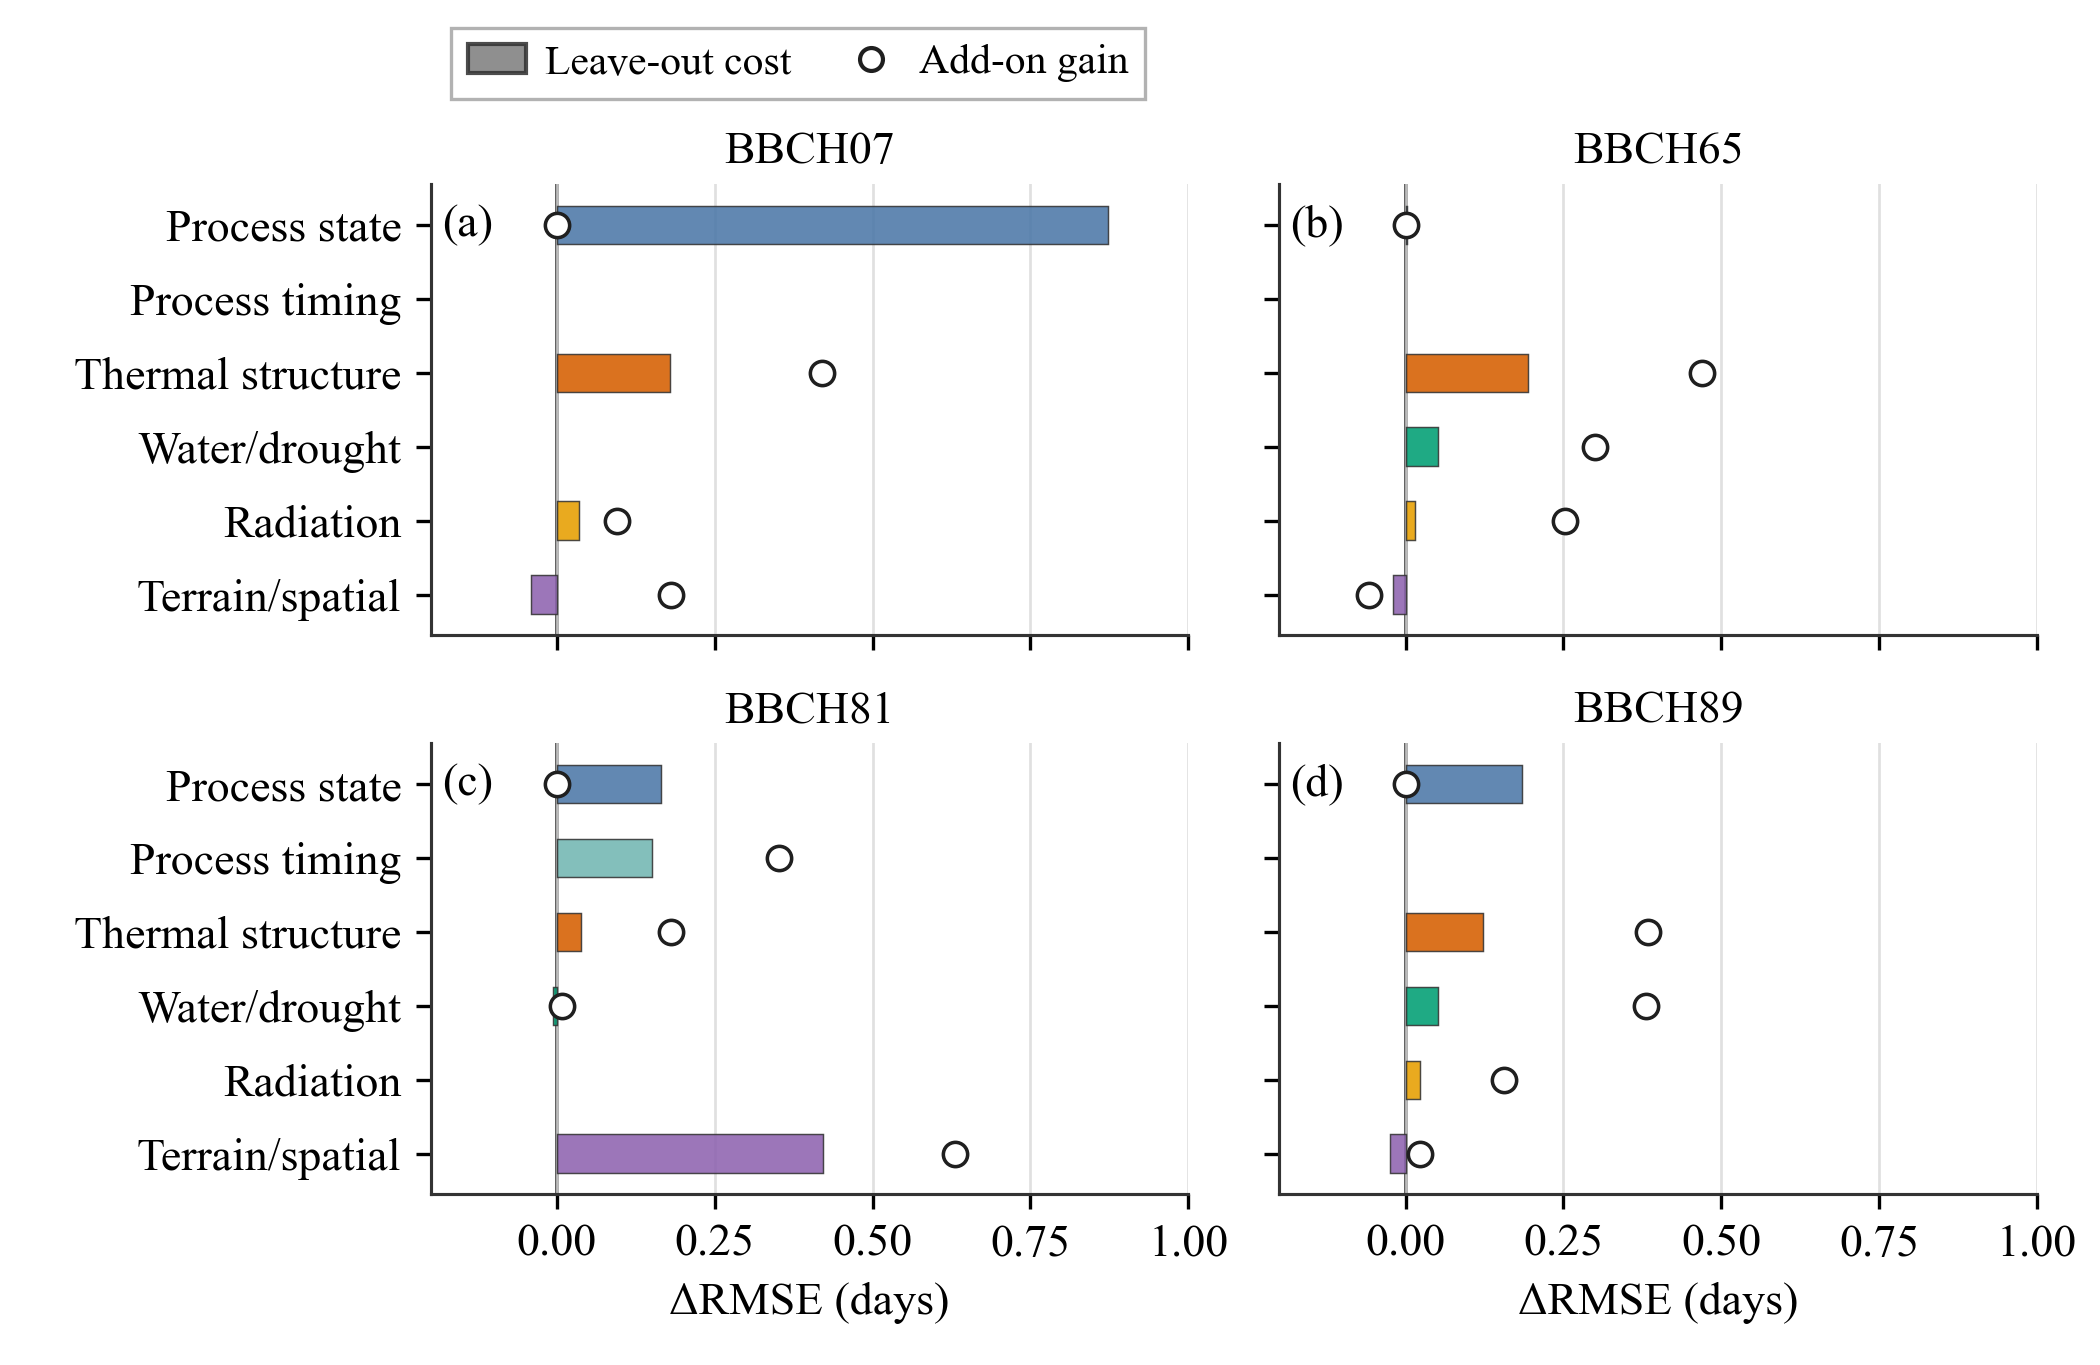
\includegraphics[width=\textwidth]{fig/results_figure/main_final_mechanism_group_ablation.png}
\caption{Mechanism-group ablation results for residual-learning features in the best hybrid models. Positive values indicate that removing the feature group worsens model performance.}
\label{fig:mechanism_group_ablation}
\end{figure}

\begin{figure}[!htbp]
\centering
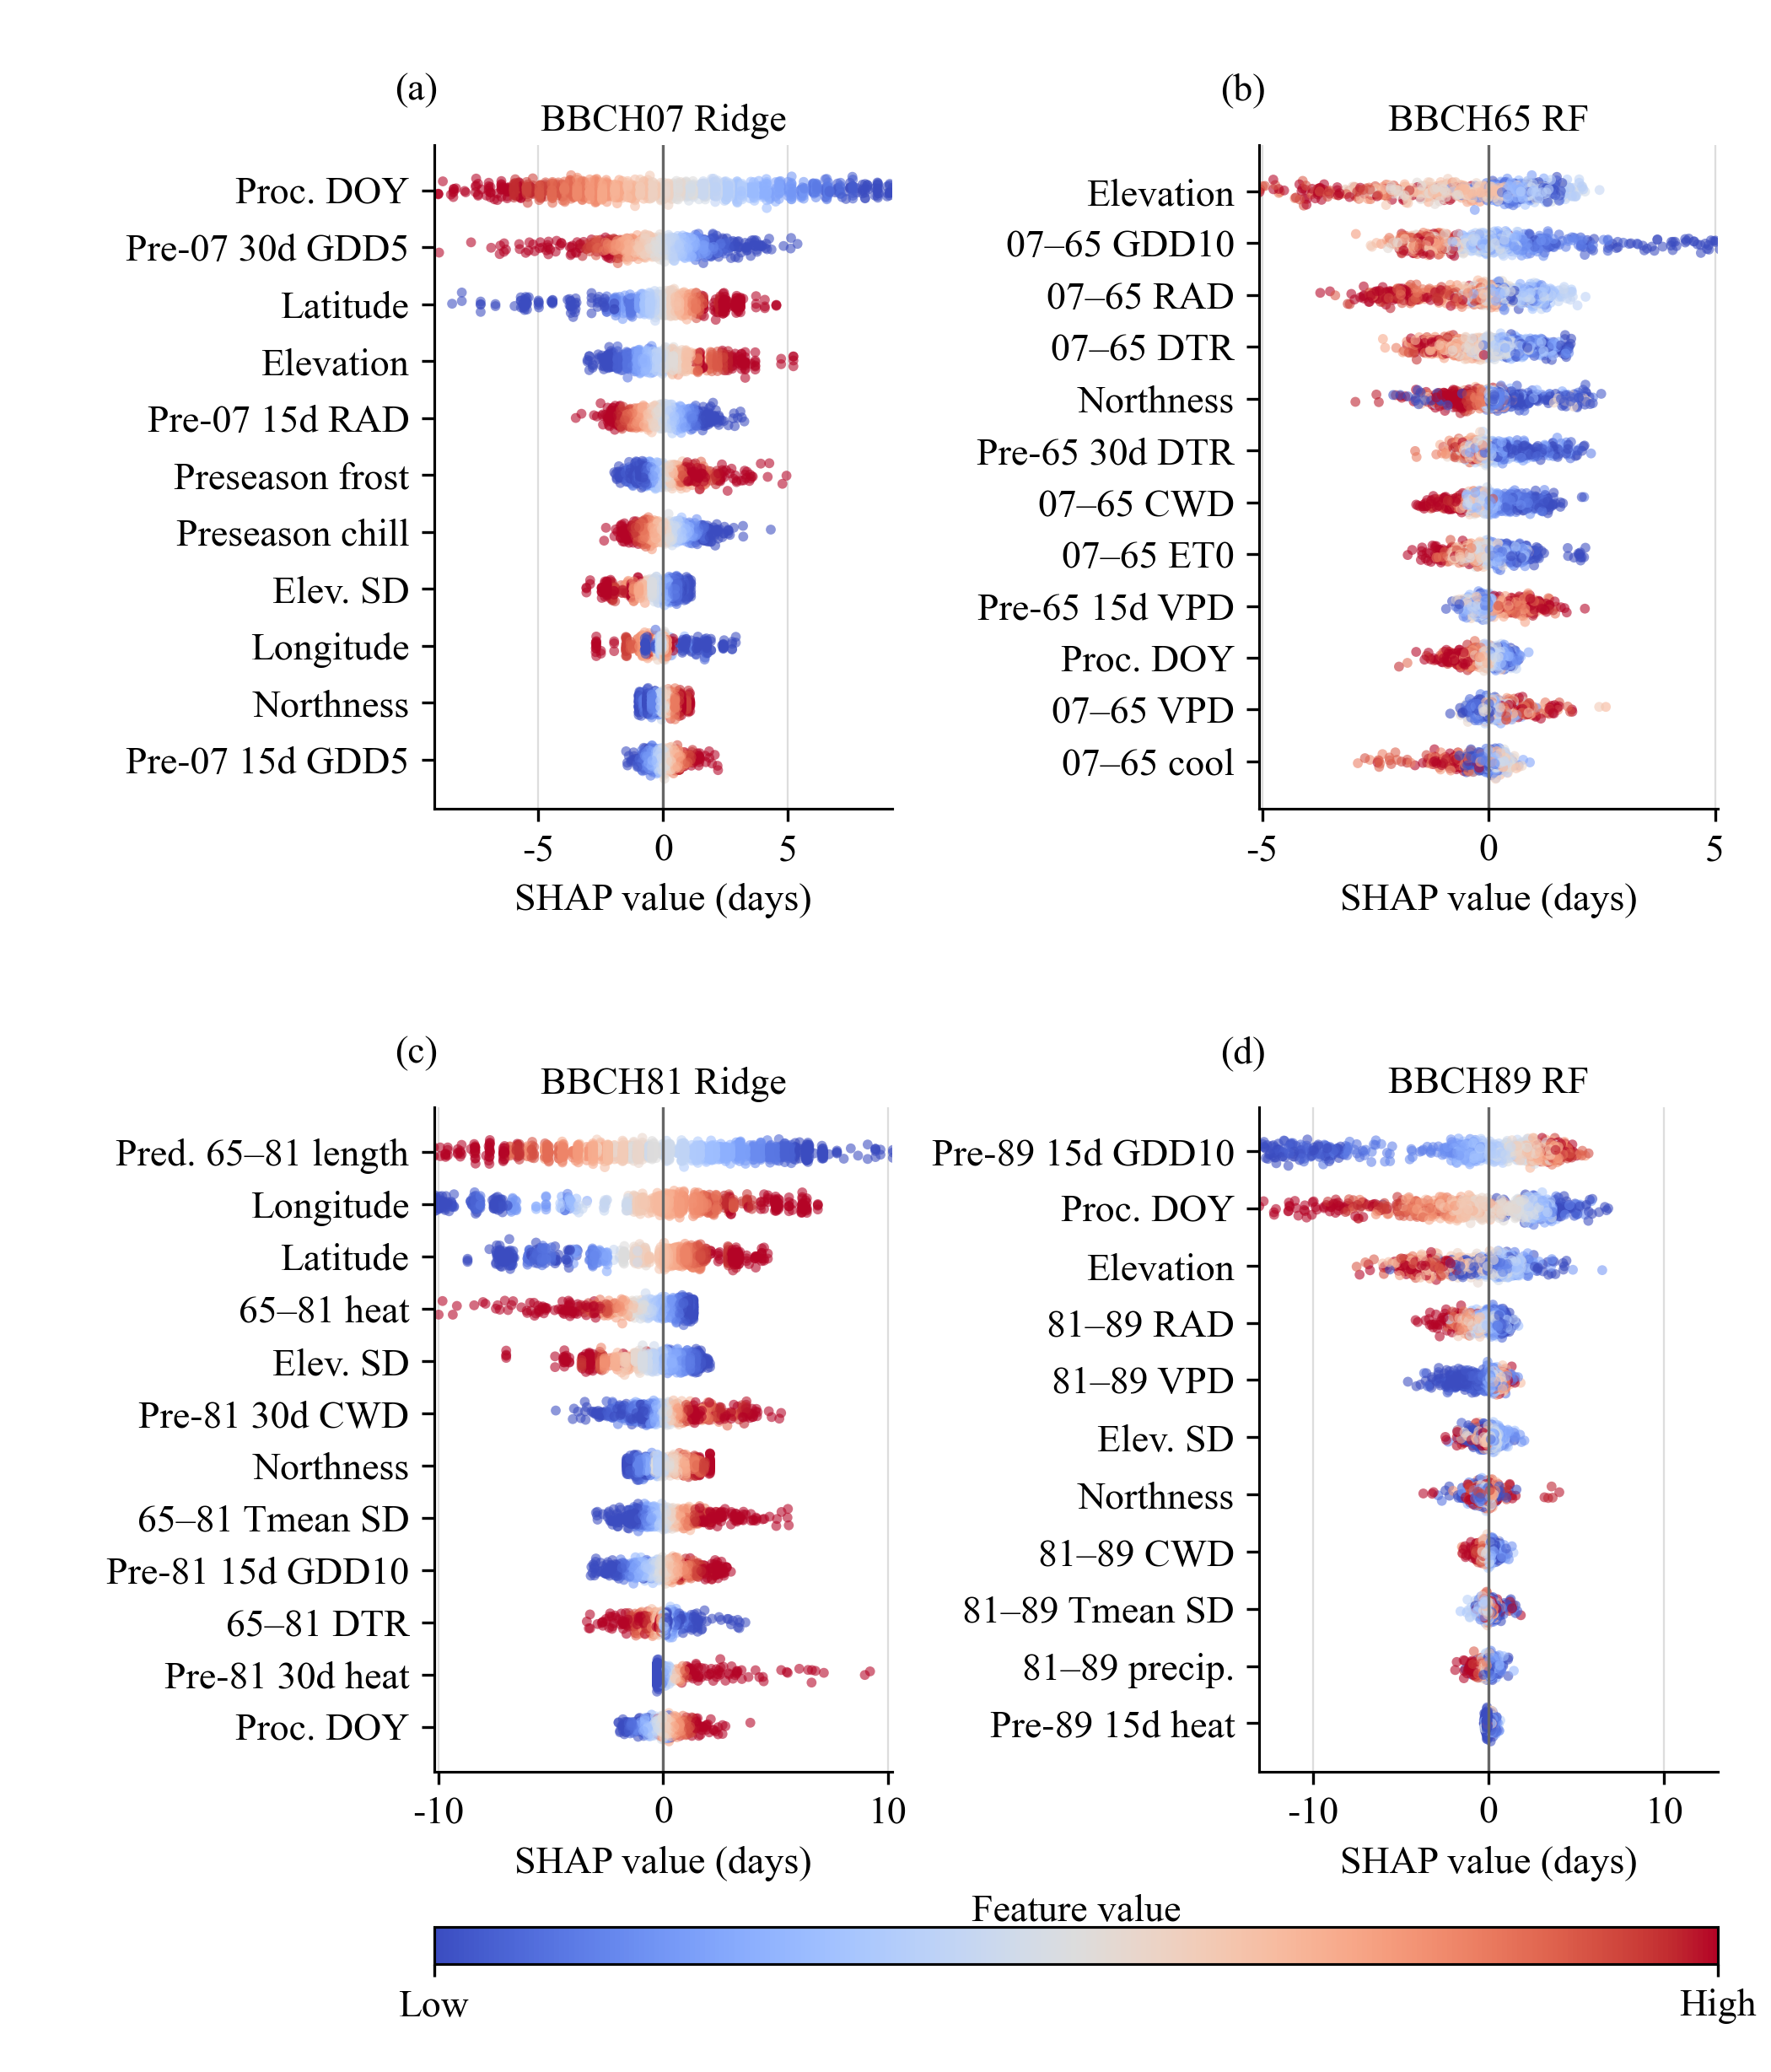
\includegraphics[width=\textwidth]{fig/results_figure/fixed_hybrid_residual_shap_all_features_beeswarm.png}
\caption{SHAP results for residual-learning features in the best hybrid models. Point color represents normalized feature values, with blue denoting low values and red denoting high values. Abbreviations: Proc. DOY, process-model predicted day of year. Pre-07/65/81/89, windows before the predicted dates of BBCH07/65/81/89. GDD, growing degree days. RAD, solar radiation. DTR, diurnal temperature range. CWD, positive climatic water deficit. VPD, vapour pressure deficit. ET0, reference evapotranspiration. SD, standard deviation.}
\label{fig:shap_residual_beeswarm}
\end{figure}

\FloatBarrier
\endgroup
\clearpage
\section{Discussion}

\begingroup
\setlength{\parindent}{0pt}
\setlength{\parskip}{0.5\baselineskip}

\subsection{Stage-dependent cross-regional transferability of process models}

Strict validation in spatially unseen areas showed that the cross-regional transferability of process models was strongly stage-dependent. BBCH07 and BBCH65 were relatively stable, suggesting that the dominant temperature-related signals during early development were sufficiently strong to support spatially independent prediction. Budburst depends on dormancy release after chilling requirements are met and subsequent heat accumulation, whereas flowering is closely linked to accumulated heat after vegetative growth resumes \citep{chuineUnifiedModelBudburst2000,garciadecortazar-atauriPerformanceSeveralModels2009,zapataPredictingKeyPhenological2017}. In addition, these stages have comparatively clear field definitions, which reduces uncertainty in the observational target. This does not imply that early phenology is free from local controls, because frost, cultivar differences and spring temperature variability can still modify event timing \citep{kellerWarmSpringTemperatures2010,cameronEffectTemperatureGrapevine2022}.

BBCH81 showed intermediate performance, indicating that veraison remains partly governed by heat accumulation but is less fully represented by a single temperature-driven process structure. Veraison marks the onset of berry ripening and can be affected by preceding developmental duration, heat exposure, water status and source--sink relations, which may reduce model transferability across regions \citep{sadrasNonlinearEffectsElevated2013,zapataPredictingKeyPhenological2017,vanleeuwenClimateChangeImpacts2024}. BBCH89 was the most difficult stage for process-only modelling, consistent with previous work showing that harvest timing is strongly affected by management-related conventions and therefore departs from a purely biological threshold \citep{ortega-fariasModelingPhenologyFour2019}. This explains why the stage-to-stage GDD10 model reduced part of the late-season bias but still produced large spatially held-out errors \citep{molitorHighResolutionCumulativeDegree2014,tomasiGrapevinePhenologyClimate2011}. Accordingly, cross-regional phenology prediction should be evaluated stage by stage under blocked spatial validation, rather than inferred from a single model structure or random cross-validation results \citep{robertsCrossvalidationStrategiesData2017,valaviBlockCVPackageGenerating2019}.

\subsection{Stage-Dependent Effects of Terrain-Adjusted Temperature}

The magnitude of terrain-based temperature correction varied spatially, rather than representing a uniform temperature shift across the study region. This pattern is consistent with the known sensitivity of vineyard microclimate to elevation, slope exposure and local terrain configuration \citep{alikadicImpactClimateChange2019,fragaModellingClimateChange2016,verdugo-vasquezEmpiricalModelEstimate2020}. The predictive value of temperature correction followed a clear stage-dependent pattern. For BBCH07 and BBCH65, terrain adjustment produced only small changes in process-model performance, likely because both stages occur early in the annual phenological sequence and budburst in particular is not controlled by heat accumulation alone. Budburst depends on dormancy release after chilling requirements are met and subsequent forcing, whereas flowering is closely related to heat accumulation after vegetative growth resumes \citep{chuineUnifiedModelBudburst2000,garciadecortazar-atauriPerformanceSeveralModels2009,zapataPredictingKeyPhenological2017}. As a result, the effect of a first-order elevation correction may have less time to accumulate in these early stages than in later seasonal windows. In contrast, BBCH81 and BBCH89 showed larger RMSE reductions after correction. Later phenological stages integrate thermal conditions over longer seasonal windows, so small daily temperature differences can accumulate into larger differences in predicted timing \citep{tomasiGrapevinePhenologyClimate2011,molitorHighResolutionCumulativeDegree2014}. This effect becomes more evident in models using longer accumulation periods or stage-to-stage late-season forcing, where terrain-related temperature mismatch can propagate through the thermal clock. The magnitude of the correction effect also differed among candidate model structures within the same stage. The contribution of this analysis is therefore not to restate that terrain affects temperature, but to quantify whether an elevation-aware correction improves phenology prediction when evaluated in unseen spatial blocks.

\subsection{Spatially Stable Residual Correction and Interpretable Signals}

Residual learning provided a correction layer that transferred to unseen spatial blocks. The fixed hybrid models reduced RMSE in all four phenological stages, from 9.6 to 8.3~d for BBCH07, from 8.2 to 7.7~d for BBCH65, from 15.5 to 14.6~d for BBCH81, and from 30.5 to 10.6~d for BBCH89. Gains were moderate for BBCH07--81, whereas BBCH89 showed a much larger improvement because the process-only model retained a strong systematic late-season bias. The near-removal of this directional offset indicates that the selected machine-learning model corrected a systematic component of the late-season error, rather than only reducing random dispersion. This is consistent with the fact that maturity or harvest timing combines biological ripening with ripeness criteria, management decisions and water-related constraints that are not explicitly represented in temperature-driven process models \citep{ortega-fariasModelingPhenologyFour2019,molitorHighResolutionCumulativeDegree2014,vanleeuwenClimateChangeImpacts2024}. MAE and RMSE decreased in every held-out outer test set, and the worst outer-round RMSE also improved. Because these gains were obtained under strict spatial separation, their consistency indicates that the machine-learning residual correction captured spatially transferable error structure rather than only local or fold-specific patterns.

The similar and moderate performance of different machine-learning algorithms for BBCH07--81 is expected under this validation setting. When the process model already captures most of the dominant phenological signal, the remaining residual target becomes smaller, noisier and harder to predict. Strict spatial separation further prevents flexible machine-learning algorithms from relying on local spatial similarity, so added model complexity does not automatically translate into stronger out-of-region performance. This explains why relatively simple models such as Ridge regression remained competitive. For BBCH89, the residuals contained a larger systematic component, and the random forest correction substantially reduced the late-stage bias.

Ablation and SHAP analyses provided evidence for interpretable residual signals \citep{lundbergUnifiedApproachInterpreting2017}. Process-model predicted timing was important in BBCH07 and BBCH89, indicating that the baseline process prediction itself carried information about residual direction and magnitude. Temperature-structure, terrain/spatial, water-demand and radiation variables contributed in a stage-specific manner, suggesting that the residuals reflected environmental and spatial information not fully represented by the temperature-driven process models. These patterns are consistent with the view that process-model residuals can contain structured information related to missing processes, input limitations or environmental gradients \citep{feiglLearningMistakesAssessing2022,reichsteinDeepLearningProcess2019,shahhosseiniCouplingMachineLearning2021}. Thus, the residual-learning component captured systematic, stage-specific environmental and spatial signals that complemented the selected process models under strict spatial extrapolation.

\subsection{Limitations and Implications}

Several limitations should be noted. First, cultivar information, management records and harvest criteria were not consistently available across the French and German datasets. This limitation is most relevant for BBCH89, because the observed date can reflect both biological maturity and operational harvest decisions. Second, the water-related predictors were based on proxy variables. VPD, ET0 and positive climatic water deficit describe atmospheric water demand, but they do not directly measure soil-water availability or vine water status. Third, terrain correction was applied to temperature using a fixed lapse-rate formulation. This provided a transparent first-order correction, but could not fully reproduce cold-air drainage, slope exposure, canopy environment or other vineyard-scale microclimatic processes. These limitations do not undermine the main inference because the study was designed to test regional spatial transferability using consistently available phenology, terrain and gridded-weather information. Future improvements will likely depend on more detailed cultivar and management records, direct soil or vine water-status information, and higher-resolution microclimatic forcing, which would allow the respective contributions of process-model structure, temperature representation and residual correction to be quantified more precisely.

\endgroup

\section{Conclusions}

\begingroup
\setlength{\parindent}{0pt}
\setlength{\parskip}{0.5\baselineskip}

This study evaluated three linked components of regional grapevine phenology prediction: the spatial transferability of process-based models across phenological stages, the practical value of terrain-adjusted temperature forcing, and the accuracy and spatial stability of hybrid models based on machine-learning residual correction. Process-model performance showed a clear stage-dependent pattern: budburst and flowering were relatively stable in unseen spatial partitions, veraison showed intermediate performance, and maturity/harvest was the most difficult stage for process-only modelling. Terrain-adjusted temperature produced quantifiable, stage-dependent improvements. Effects were small for BBCH07 and BBCH65, but larger for BBCH81 and BBCH89. Under strict spatial validation, residual learning further improved prediction accuracy for all four phenological stages and nearly removed the late-season directional bias, with gains remaining stable across the five held-out outer test sets. Mechanism-group ablation and SHAP analyses showed that residual corrections were associated with process-model-predicted timing, temperature structure, terrain/spatial, water-demand and radiation signals. Overall, this study improves the reliability of regional grapevine phenology prediction and provides a process-model and machine-learning residual-correction framework for vineyard management under complex terrain and heterogeneous climate conditions.

\endgroup

\section*{CRediT authorship contribution statement}

\section*{Declaration of competing interest}
The authors declare that they have no known competing financial interests or personal relationships that could have appeared to influence the work reported in this paper.

\section*{Acknowledgements}

\section*{Data availability}
The data supporting the findings of this study are available from the corresponding author upon reasonable request, subject to the original data providers' terms.

\bibliographystyle{plainnat}
\bibliography{references/Phenological}

\end{document}
